\documentclass[11pt,a4paper]{article}

% Packages
\usepackage[utf8]{inputenc}
\usepackage[T1]{fontenc}
\usepackage{amsmath,amssymb}
\usepackage{graphicx}
\usepackage{booktabs}
\usepackage{hyperref}
\usepackage[margin=1in]{geometry}
\usepackage{caption}
\usepackage{subcaption}
\usepackage{listings}
\usepackage{xcolor}
\usepackage{float}

% Code listing style
\lstset{
    basicstyle=\ttfamily\small,
    breaklines=true,
    frame=single,
    backgroundcolor=\color{gray!10},
    keywordstyle=\color{blue},
    commentstyle=\color{green!50!black},
}

\title{SL-GPS Validation Report:\\Multi-Fuel Mechanism Reduction\\via Supervised Learning}
\author{SL-GPS Automated Validation Framework}
\date{\today}

\begin{document}

\maketitle

\begin{abstract}
This report presents a systematic validation of the Supervised Learning -- Global Pathway Selection (SL-GPS) method for adaptive chemical mechanism reduction using AramcoMech 3.0 (581 species, 3037 reactions). Three fuels are studied: methane (CH$_4$), propane (C$_3$H$_8$), and ethylene (C$_2$H$_4$). For each fuel, the complete pipeline is documented: training data generation via GPS, neural network training, and validation against the detailed mechanism across 4--8 test cases spanning wide temperature, pressure, and equivalence ratio ranges. All training parameters, species classifications, epoch histories, and computational costs are reported to enable full reproducibility.
\end{abstract}

\tableofcontents
\newpage

% =============================================================================
\section{Introduction}
% =============================================================================

The SL-GPS method trains neural networks on Global Pathway Selection (GPS) data to dynamically predict which chemical species are important during combustion simulations. At each timestep, the ANN evaluates the current thermochemical state and activates only the predicted species, producing an adaptive reduced mechanism that varies in size throughout the simulation.

This report validates SL-GPS on AramcoMech 3.0 \cite{aramco3} (581 species, 3037 reactions) across three fuels of increasing complexity:
\begin{itemize}
    \item \textbf{Methane (CH$_4$)} --- baseline single-carbon fuel
    \item \textbf{Propane (C$_3$H$_8$)} --- multi-carbon alkane
    \item \textbf{Ethylene (C$_2$H$_4$)} --- alkene with different pathway structures
\end{itemize}

Each fuel study is self-contained (Sections~\ref{sec:ch4}--\ref{sec:c2h4}) and follows a consistent structure: training configuration, species classification, validation cases, per-case results, summary, and timing.

% =============================================================================
\section{Common Methodology}
\label{sec:methodology}
% =============================================================================

\subsection{SL-GPS Pipeline}

The pipeline for each fuel consists of three stages:
\begin{enumerate}
    \item \textbf{Data generation:} Run $N$ autoignition simulations with randomized initial conditions ($T$, $P$, composition). At each timestep interval, apply GPS ($\alpha = 0.001$) to label which species are important.
    \item \textbf{ANN training:} Train an ensemble of neural networks on the GPS-labeled data. Select the best model by validation loss.
    \item \textbf{Validation:} Run new autoignition cases with the detailed mechanism and simultaneously with SL-GPS (ANN-guided reduction). Compare temperature, HRR, species profiles, and ignition delay.
\end{enumerate}

\subsection{Species Classification}

Before training, species are partitioned into three groups based on occurrence frequency in the GPS training data:
\begin{itemize}
    \item \textbf{Always} ($>99\%$ occurrence): unconditionally included in all reduced mechanisms
    \item \textbf{Variable} (1--99\%): predicted by the ANN at each timestep
    \item \textbf{Never} ($<1\%$ occurrence): permanently excluded
\end{itemize}
Only the \emph{variable} species are outputs of the neural network.

\subsection{Neural Network Architecture}

All models use the same general architecture:
\begin{itemize}
    \item \textbf{Input:} temperature, pressure, and selected species mole fractions (normalized via MinMaxScaler)
    \item \textbf{Hidden layers:} 2 fully-connected layers with ReLU activation
    \item \textbf{Output:} sigmoid activation (one output per variable species)
    \item \textbf{Loss:} binary cross-entropy; \textbf{Optimizer:} Adam
    \item \textbf{Training:} ensemble of 8 models in parallel, best selected by validation loss
    \item \textbf{Early stopping:} patience = 30 epochs, max = 200 epochs
\end{itemize}

\subsection{Validation Metrics}

For each validation case, we report:
\begin{itemize}
    \item Temperature and heat release rate profiles (detailed vs.\ SL-GPS)
    \item Major species evolution
    \item Mechanism size (active species count) over time
    \item Ignition delay error
    \item Computational timing: chemistry solve time vs.\ ANN evaluation time
\end{itemize}

% =============================================================================
% =============================================================================
\newpage
\section{Methane (CH\texorpdfstring{$_4$}{4}) --- AramcoMech 3.0}
\label{sec:ch4}
% =============================================================================
% =============================================================================

\subsection{Training Configuration}

\begin{table}[H]
\centering
\caption{CH$_4$ training configuration summary.}
\label{tab:ch4_config}
\begin{tabular}{ll}
\toprule
\textbf{Parameter} & \textbf{Value} \\
\midrule
\multicolumn{2}{l}{\textit{Mechanism}} \\
\quad Mechanism & AramcoMech 3.0 \\
\quad Species / Reactions & 581 / 3037 \\
\midrule
\multicolumn{2}{l}{\textit{Data Generation}} \\
\quad Training cases & 30 (parallel execution) \\
\quad Temperature range & 900--2000~K (uniform) \\
\quad Pressure range & 1--40~atm (log-uniform) \\
\quad Composition & randomized $X_{\text{CH}_4}$, $X_{\text{O}_2}$, $X_{\text{N}_2}$, $X_{\text{CO}_2}$, $X_{\text{H}_2\text{O}}$ \\
\quad GPS $\alpha$ & 0.001 \\
\quad Total training samples & 1451 \\
\quad Data generation time & 58.4~s \\
\midrule
\multicolumn{2}{l}{\textit{Species Classification}} \\
\quad Always species & 13 \\
\quad Variable species (ANN outputs) & 33 \\
\quad Never species & 8 \\
\midrule
\multicolumn{2}{l}{\textit{ANN Training}} \\
\quad Input features & $T$, $P$ + 10 species mole fractions \\
\quad Architecture & 2 hidden layers $\times$ 24 neurons \\
\quad Ensemble size & 8 parallel trainings \\
\quad Max epochs / Early stopping & 200 / patience 30 \\
\quad Actual epochs (best model) & 192 (early stopped) \\
\bottomrule
\end{tabular}
\end{table}

\textbf{Input species (ANN features):} CH$_4$, O$_2$, H$_2$O, CO$_2$, CO, OH, H, H$_2$, CH$_3$, HO$_2$

\subsection{Validation Cases}

\begin{table}[H]
\centering
\caption{CH$_4$ validation conditions.}
\label{tab:ch4_cases}
\begin{tabular}{lcccc}
\toprule
\textbf{Case} & \textbf{$T_0$ (K)} & \textbf{$P$ (atm)} & \textbf{$\phi$} & \textbf{$t_{\text{end}}$ (s)} \\
\midrule
CH4\_T1000\_P1 & 1000 & 1 & 1.0 & 0.1 \\
CH4\_T1500\_P1 & 1500 & 1 & 1.0 & 0.005 \\
CH4\_T1500\_P10 & 1500 & 10 & 1.0 & 0.002 \\
CH4\_T2000\_P1 & 2000 & 1 & 1.0 & 0.001 \\
\bottomrule
\end{tabular}
\end{table}

\subsection{Results}

\begin{figure}[H]
    \centering
    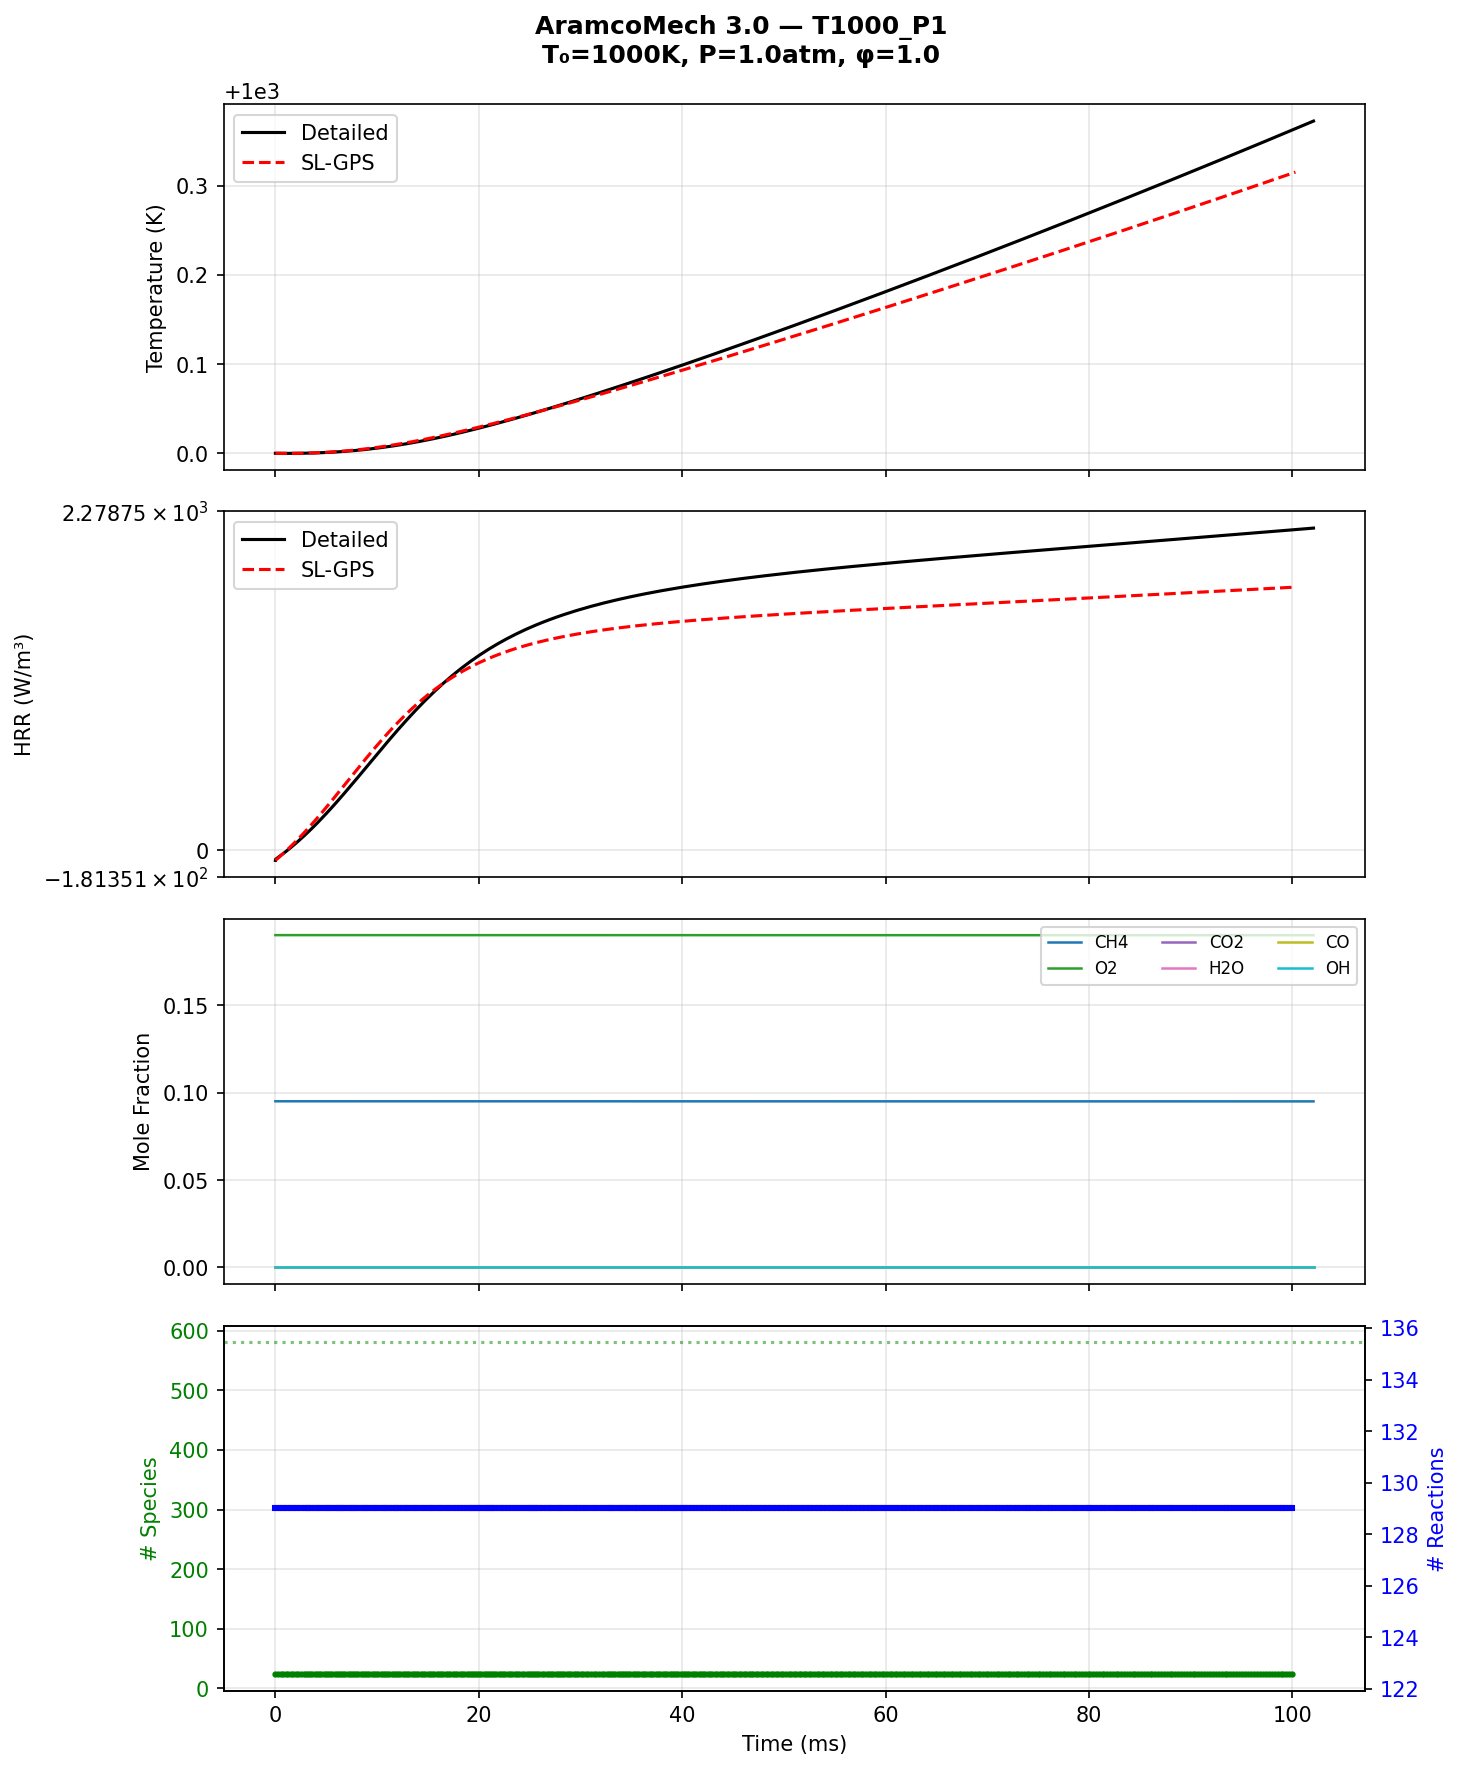
\includegraphics[width=0.95\textwidth]{results/ch4/T1000_P1.png}
    \caption{CH$_4$ Case 1: $T_0=1000$~K, $P=1$~atm, $\phi=1.0$.}
    \label{fig:ch4_case1}
\end{figure}

\begin{figure}[H]
    \centering
    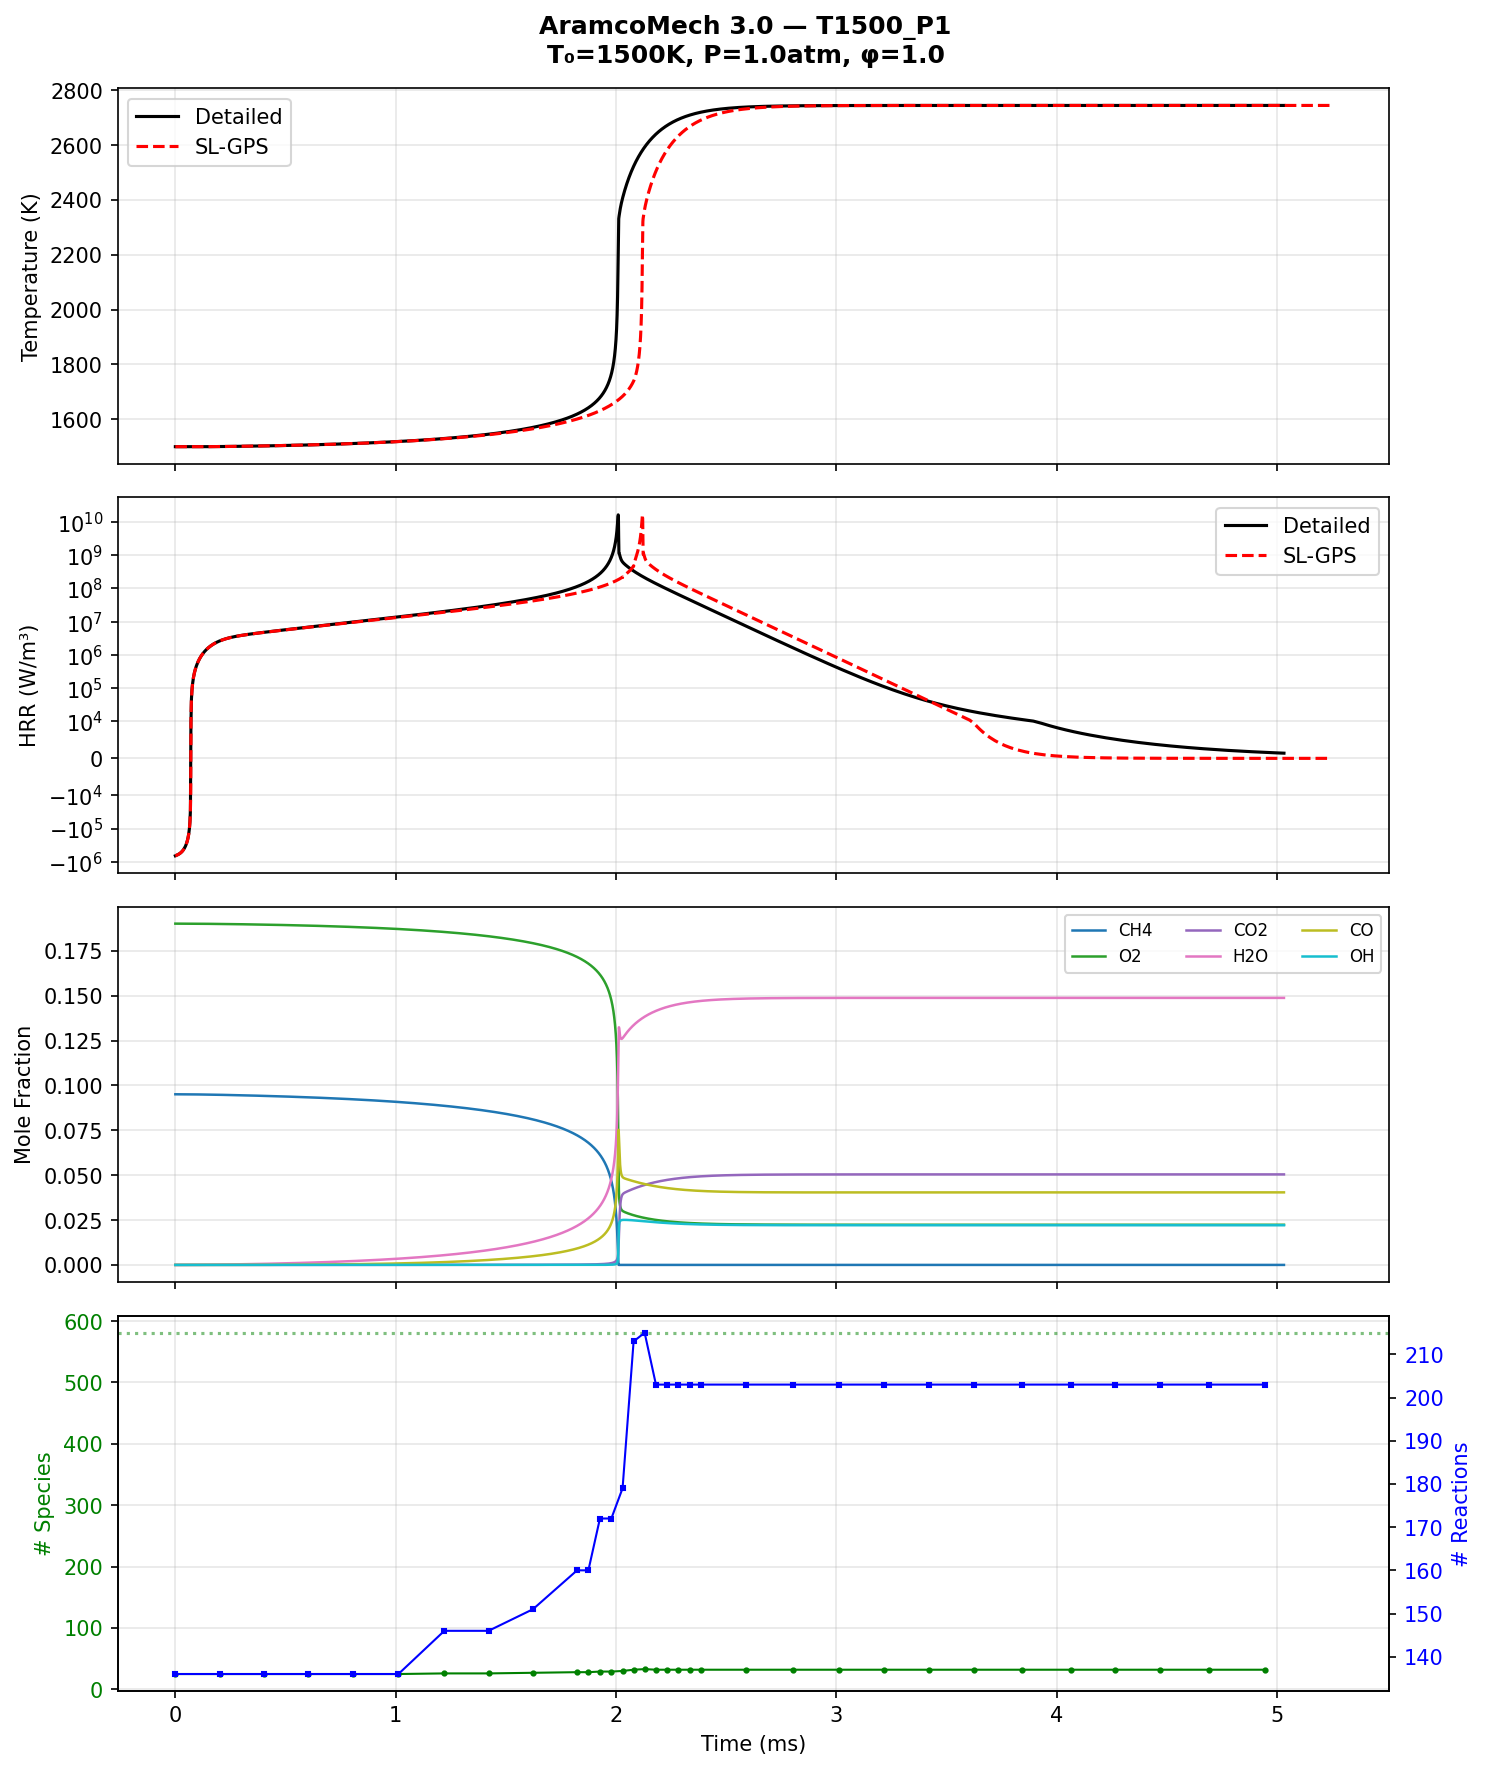
\includegraphics[width=0.95\textwidth]{results/ch4/T1500_P1.png}
    \caption{CH$_4$ Case 2: $T_0=1500$~K, $P=1$~atm, $\phi=1.0$.}
    \label{fig:ch4_case2}
\end{figure}

\begin{figure}[H]
    \centering
    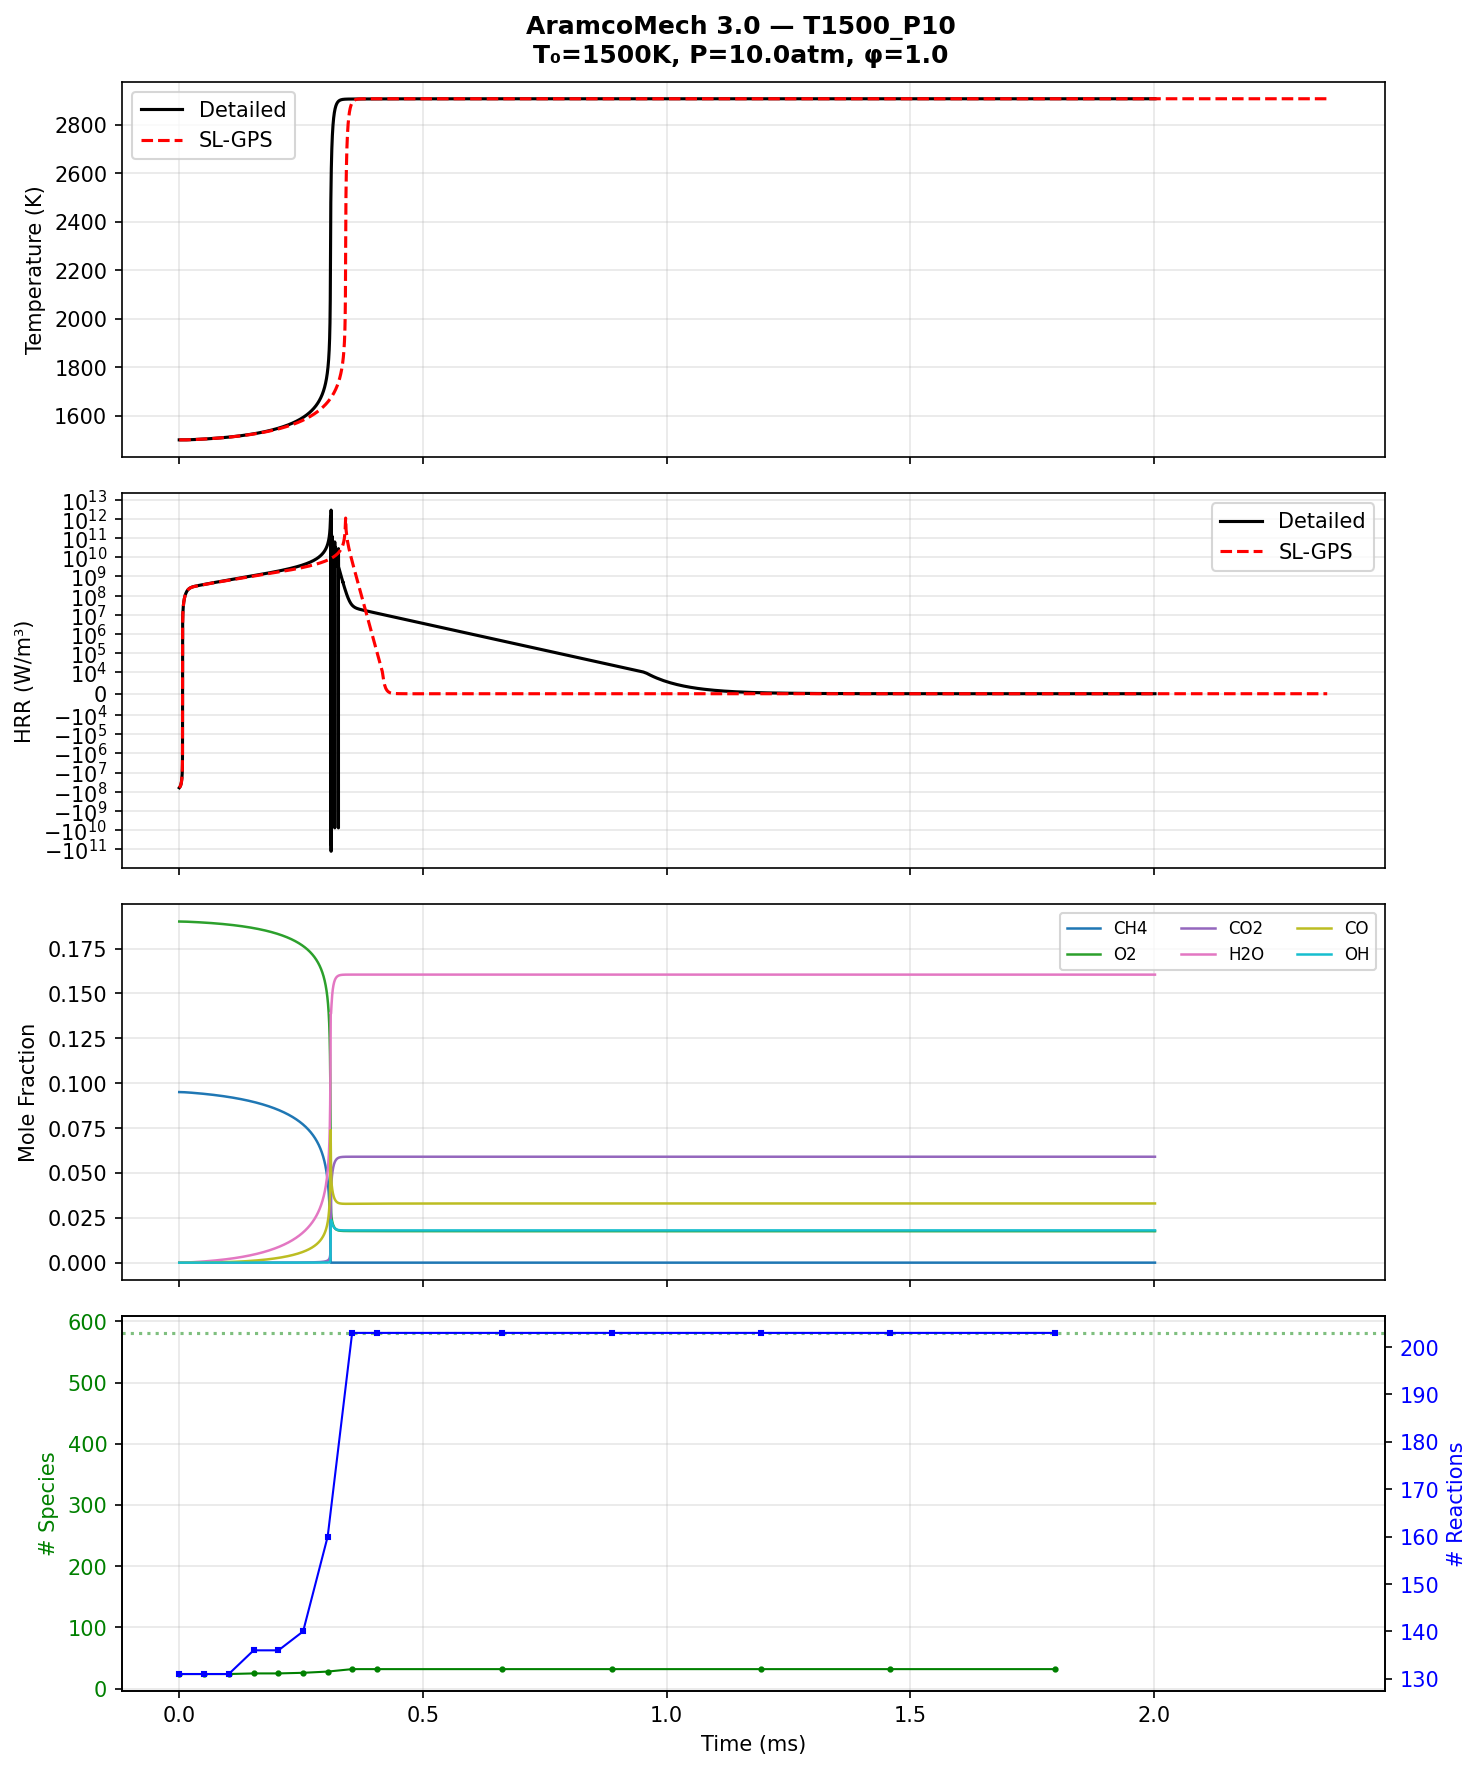
\includegraphics[width=0.95\textwidth]{results/ch4/T1500_P10.png}
    \caption{CH$_4$ Case 3: $T_0=1500$~K, $P=10$~atm, $\phi=1.0$.}
    \label{fig:ch4_case3}
\end{figure}

\begin{figure}[H]
    \centering
    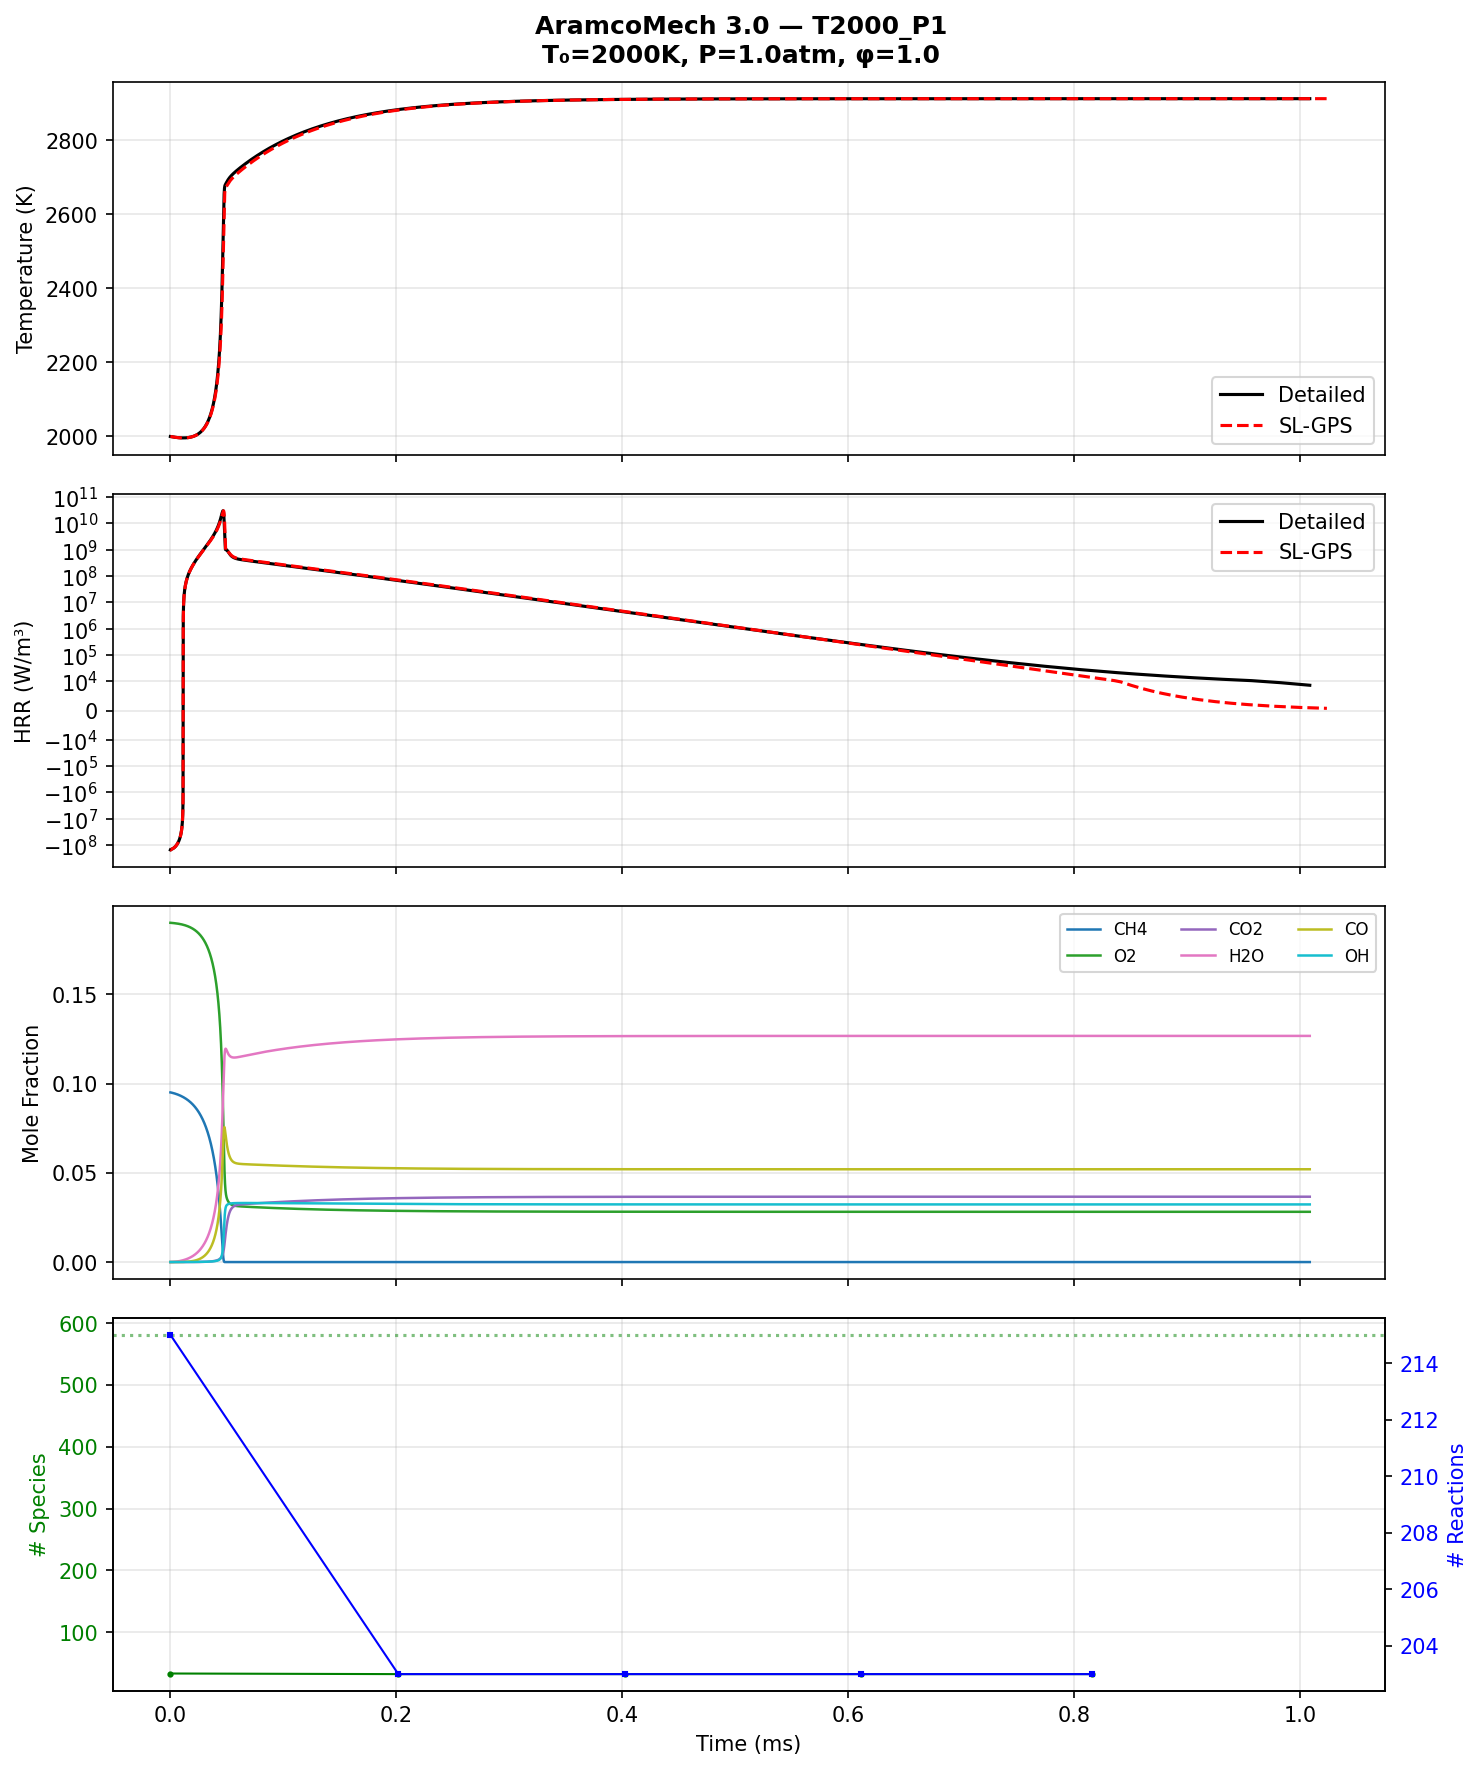
\includegraphics[width=0.95\textwidth]{results/ch4/T2000_P1.png}
    \caption{CH$_4$ Case 4: $T_0=2000$~K, $P=1$~atm, $\phi=1.0$.}
    \label{fig:ch4_case4}
\end{figure}

\subsection{Summary}

\begin{figure}[H]
    \centering
    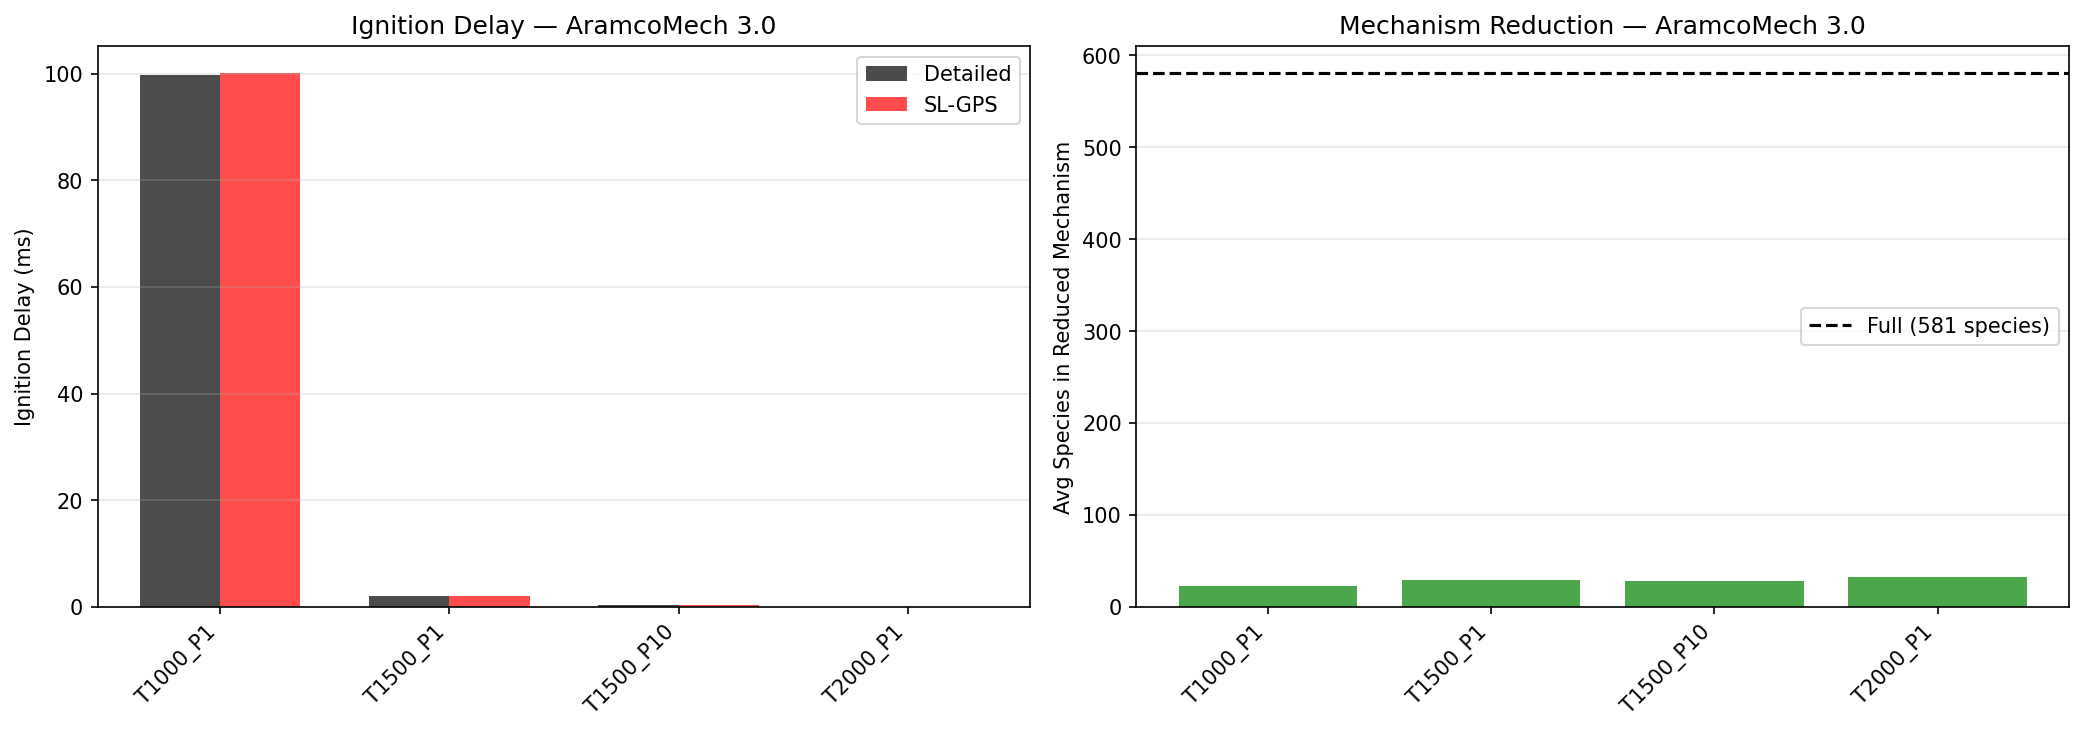
\includegraphics[width=0.95\textwidth]{results/ch4/summary.png}
    \caption{CH$_4$ validation summary. Left: ignition delay comparison. Right: average mechanism size (reduced vs.\ full 53 species).}
    \label{fig:ch4_summary}
\end{figure}

% =============================================================================
% =============================================================================
\newpage
\section{Propane (C\texorpdfstring{$_3$}{3}H\texorpdfstring{$_8$}{8}) --- AramcoMech 3.0}
\label{sec:c3h8}
% =============================================================================
% =============================================================================

\subsection{Training Configuration}

\begin{table}[H]
\centering
\caption{C$_3$H$_8$ training configuration summary.}
\label{tab:c3h8_config}
\begin{tabular}{ll}
\toprule
\textbf{Parameter} & \textbf{Value} \\
\midrule
\multicolumn{2}{l}{\textit{Mechanism}} \\
\quad Mechanism & AramcoMech 3.0 \\
\quad Species / Reactions & 581 / 3037 \\
\midrule
\multicolumn{2}{l}{\textit{Data Generation}} \\
\quad Training cases & 15 (serial execution$^*$) \\
\quad Temperature range & 900--1800~K (uniform) \\
\quad Pressure range & 1--20~atm (log-uniform) \\
\quad Equivalence ratio $\phi$ & 0.8--1.4 (uniform) \\
\quad GPS $\alpha$ & 0.001 \\
\quad Total training samples & 686 \\
\quad Data generation time & 1384.3~s (23.1~min) \\
\midrule
\multicolumn{2}{l}{\textit{Species Classification}} \\
\quad Always species & 15 \\
\quad Variable species (ANN outputs) & 222 \\
\quad Never species & 344 \\
\midrule
\multicolumn{2}{l}{\textit{ANN Training}} \\
\quad Input features & $T$, $P$ + 14 species mole fractions \\
\quad Architecture & 2 hidden layers $\times$ 32 neurons \\
\quad Ensemble size & 8 parallel trainings \\
\quad Max epochs / Early stopping & 200 / patience 30 \\
\quad Actual epochs (best model) & 141 (early stopped) \\
\quad Training time & 35.0~s \\
\bottomrule
\end{tabular}
\end{table}

\noindent$^*$\textit{Serial execution required to avoid} \texttt{multiprocessing.Pool} \textit{deadlocks (fork + Cantera C++ internals with 581-species mechanism).}

\medskip
\textbf{Input species (ANN features):} C$_3$H$_8$, O$_2$, H$_2$O, CO$_2$, CO, OH, H, H$_2$, CH$_4$, C$_2$H$_4$, C$_2$H$_6$, CH$_2$O, C$_3$H$_6$, HO$_2$

\subsection{Validation Cases}

\begin{table}[H]
\centering
\caption{C$_3$H$_8$ validation conditions (4 baseline + 4 extended).}
\label{tab:c3h8_cases}
\begin{tabular}{lcccc}
\toprule
\textbf{Case} & \textbf{$T_0$ (K)} & \textbf{$P$ (atm)} & \textbf{$\phi$} & \textbf{$t_{\text{end}}$ (s)} \\
\midrule
C3H8\_T1000\_P1 & 1000 & 1 & 1.0 & 0.2 \\
C3H8\_T1200\_P10 & 1200 & 10 & 1.0 & 0.02 \\
C3H8\_T1500\_P1 & 1500 & 1 & 1.0 & 0.005 \\
C3H8\_T1500\_P10 & 1500 & 10 & 1.0 & 0.002 \\
\midrule
\multicolumn{5}{c}{\textit{Extended cases (difficult conditions)}} \\
\midrule
C3H8\_T900\_P20 & 900 & 20 & 1.0 & 0.5 \\
C3H8\_T1200\_P1\_rich & 1200 & 1 & 1.3 & 0.05 \\
C3H8\_T1300\_P5\_lean & 1300 & 5 & 0.7 & 0.01 \\
C3H8\_T1800\_P20 & 1800 & 20 & 1.0 & 0.001 \\
\bottomrule
\end{tabular}
\end{table}

\subsection{Results --- Baseline Cases}

\begin{figure}[H]
    \centering
    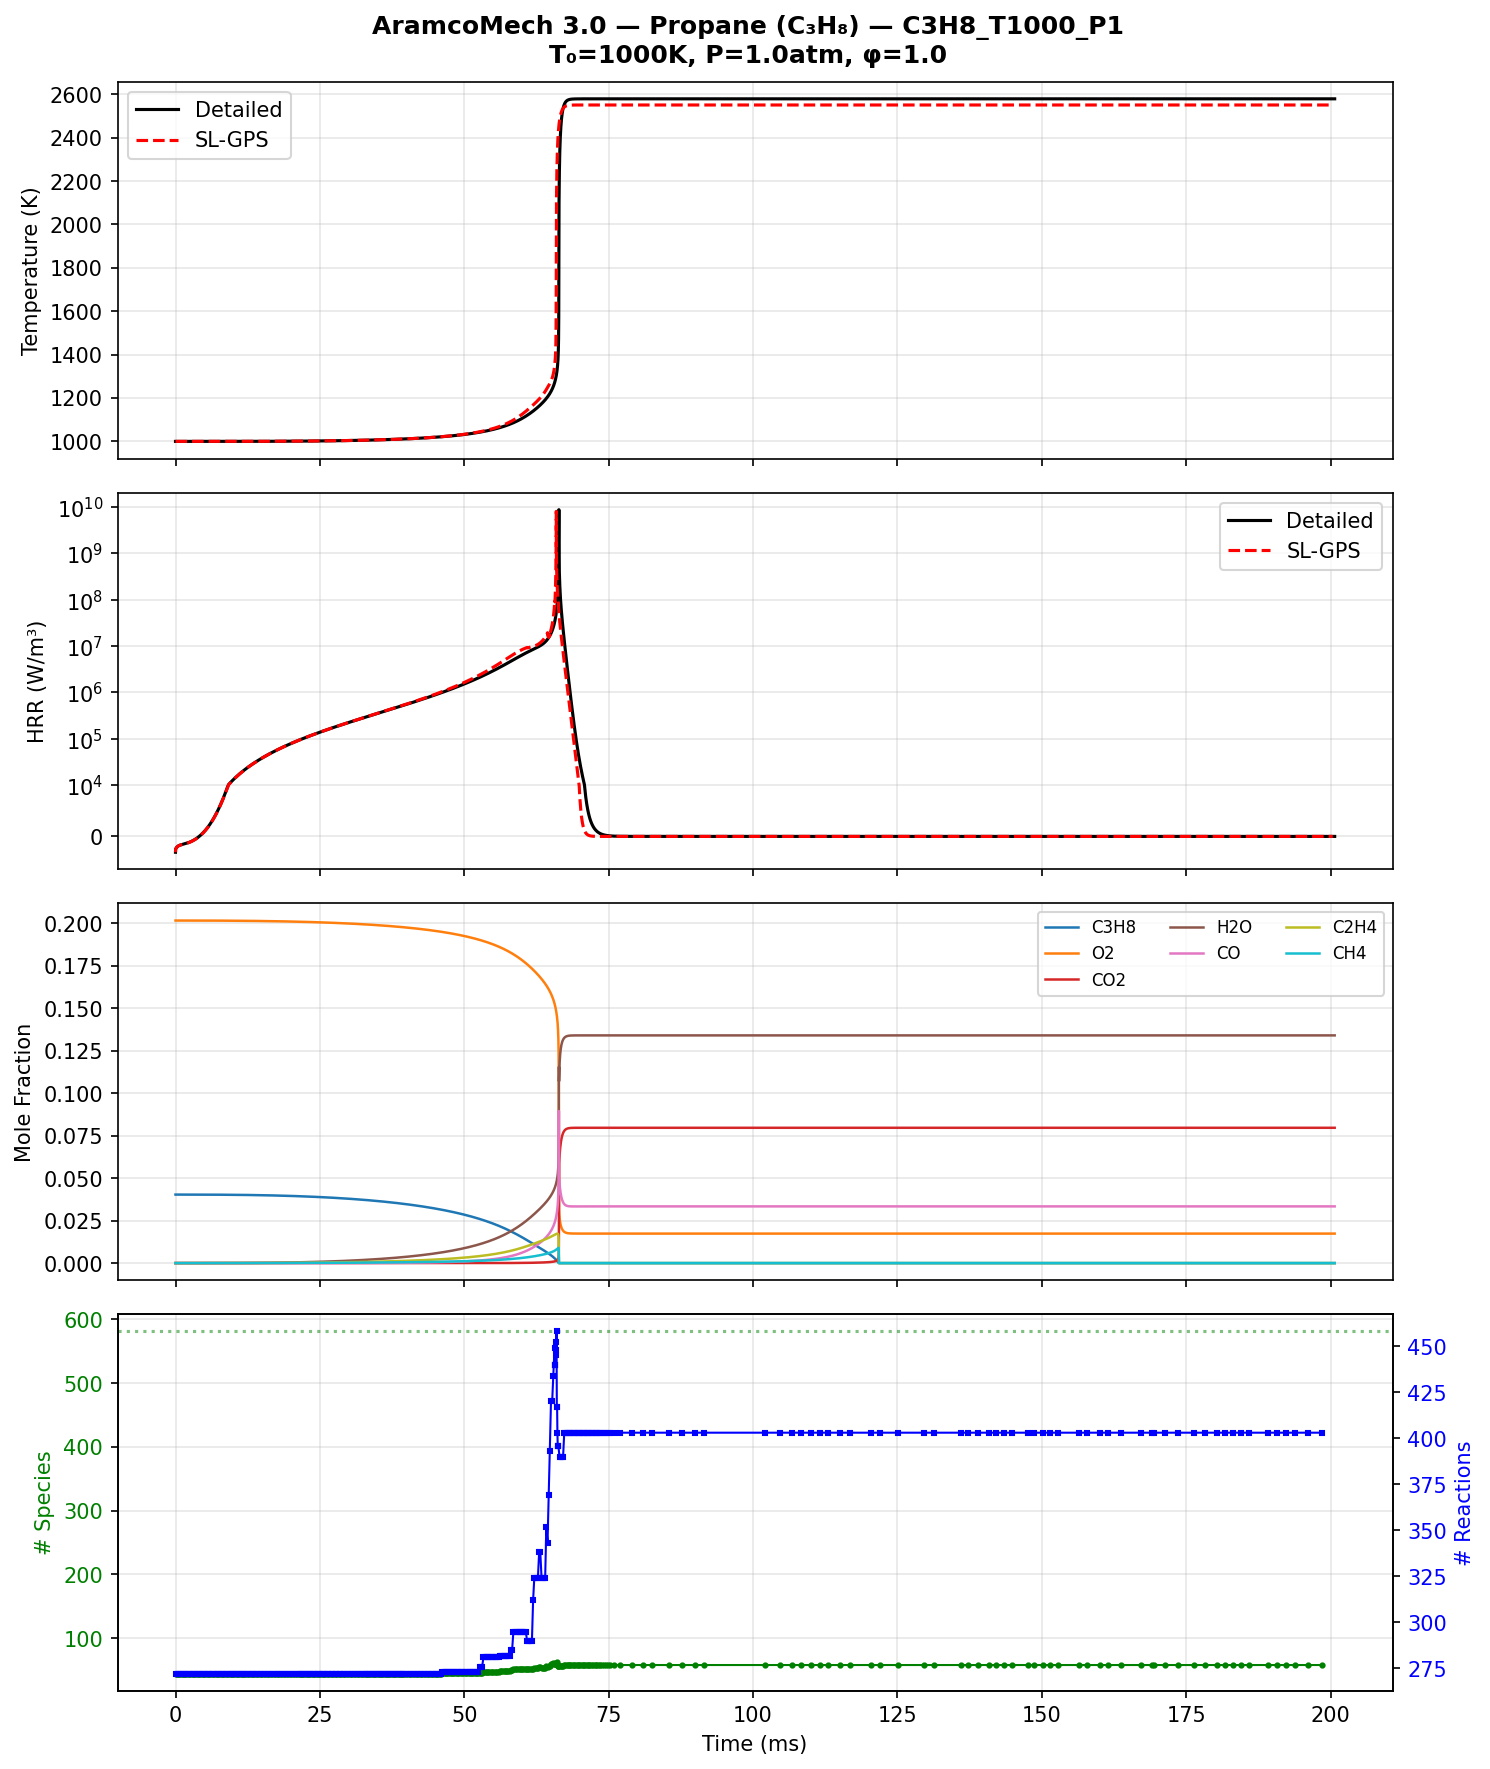
\includegraphics[width=0.95\textwidth]{results/c3h8/C3H8_T1000_P1.png}
    \caption{C$_3$H$_8$ Case 1: $T_0=1000$~K, $P=1$~atm, $\phi=1.0$.}
    \label{fig:c3h8_case1}
\end{figure}

\begin{figure}[H]
    \centering
    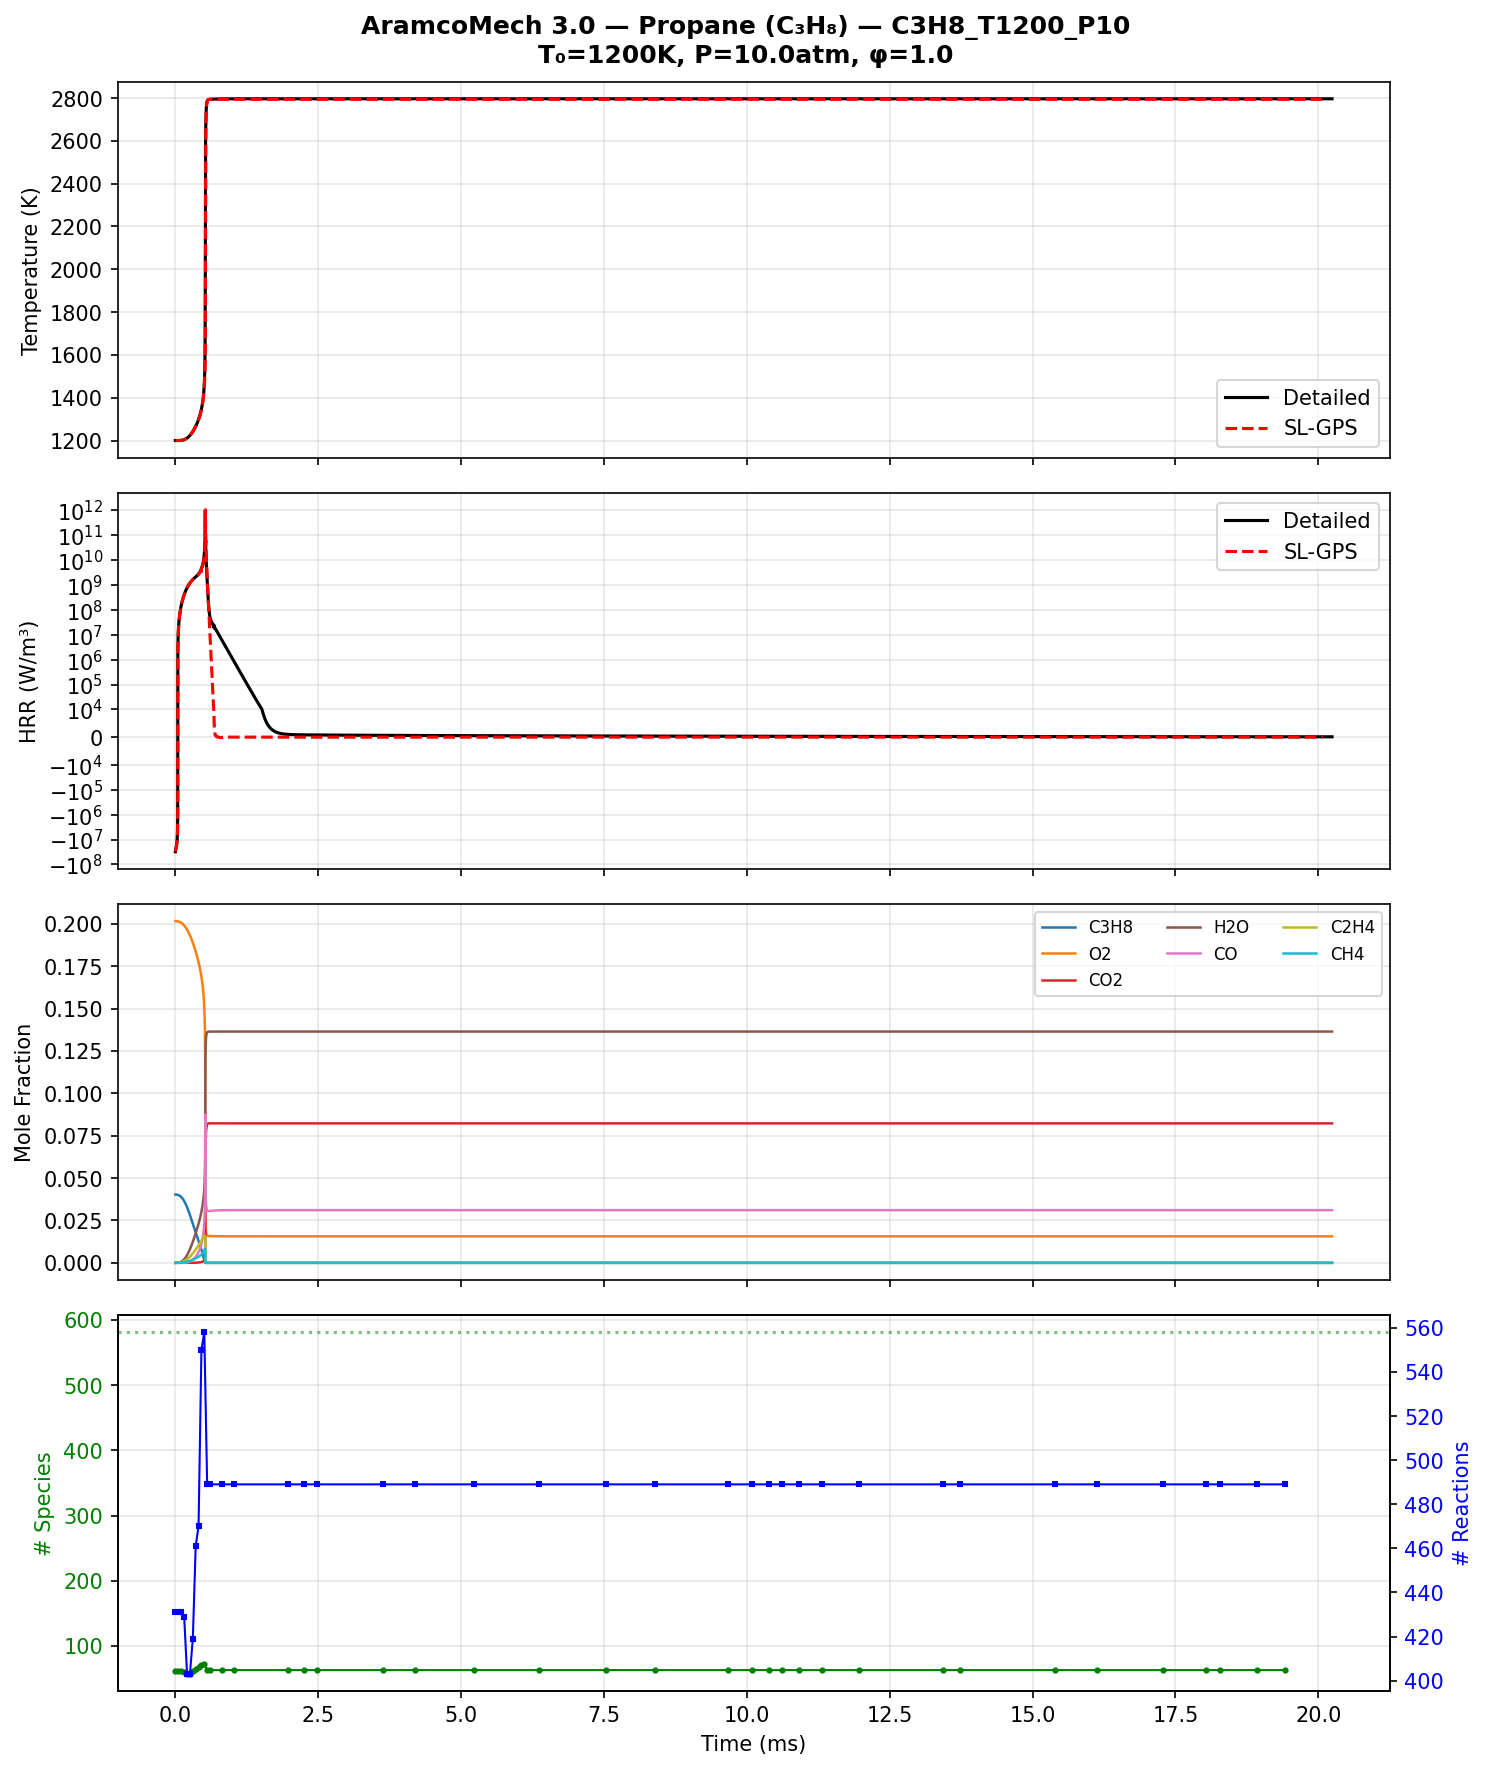
\includegraphics[width=0.95\textwidth]{results/c3h8/C3H8_T1200_P10.png}
    \caption{C$_3$H$_8$ Case 2: $T_0=1200$~K, $P=10$~atm, $\phi=1.0$.}
    \label{fig:c3h8_case2}
\end{figure}

\begin{figure}[H]
    \centering
    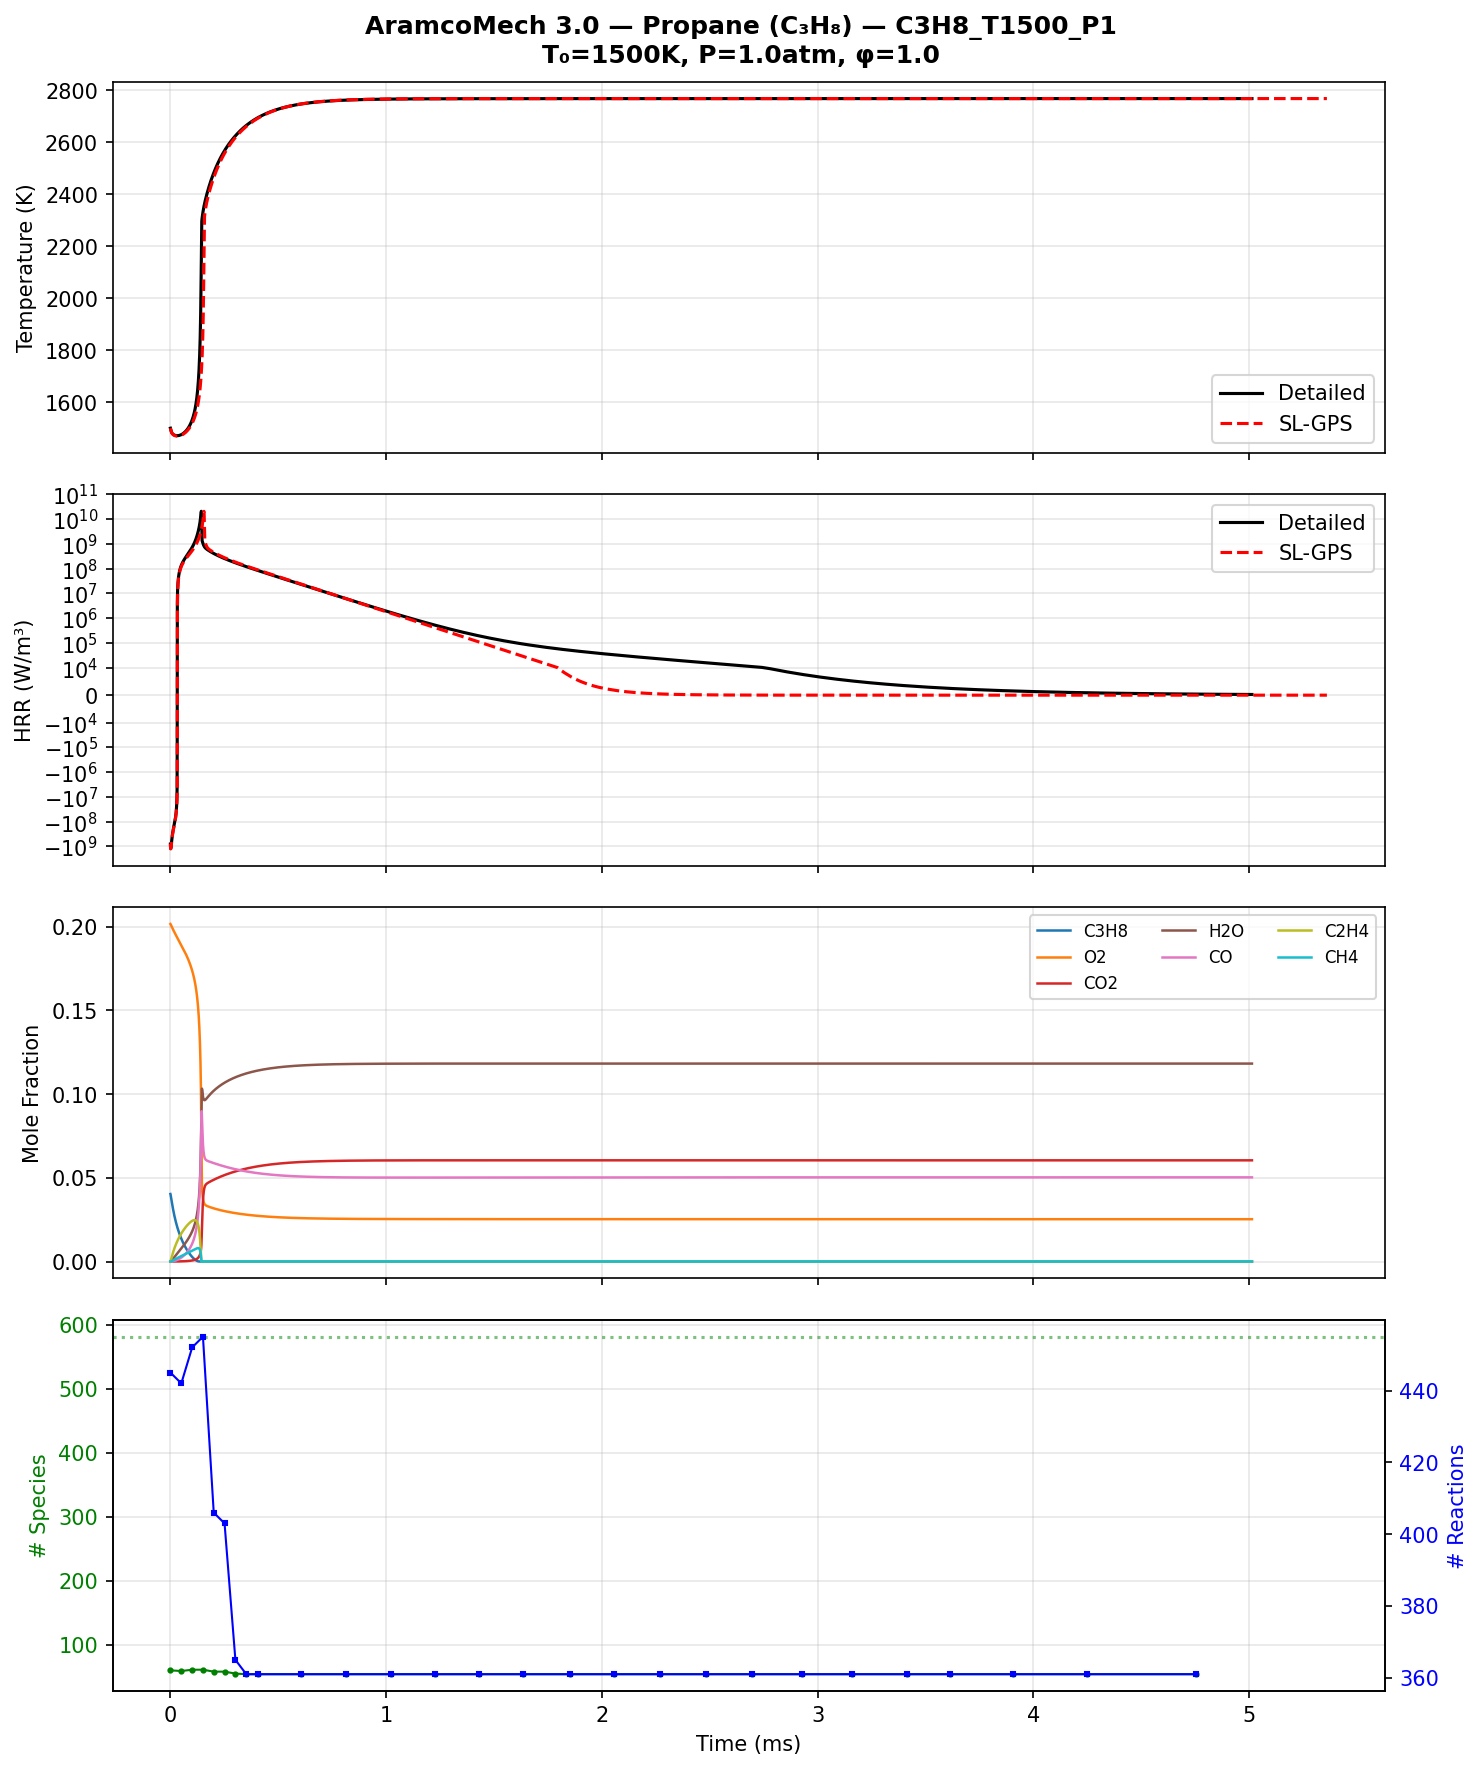
\includegraphics[width=0.95\textwidth]{results/c3h8/C3H8_T1500_P1.png}
    \caption{C$_3$H$_8$ Case 3: $T_0=1500$~K, $P=1$~atm, $\phi=1.0$.}
    \label{fig:c3h8_case3}
\end{figure}

\begin{figure}[H]
    \centering
    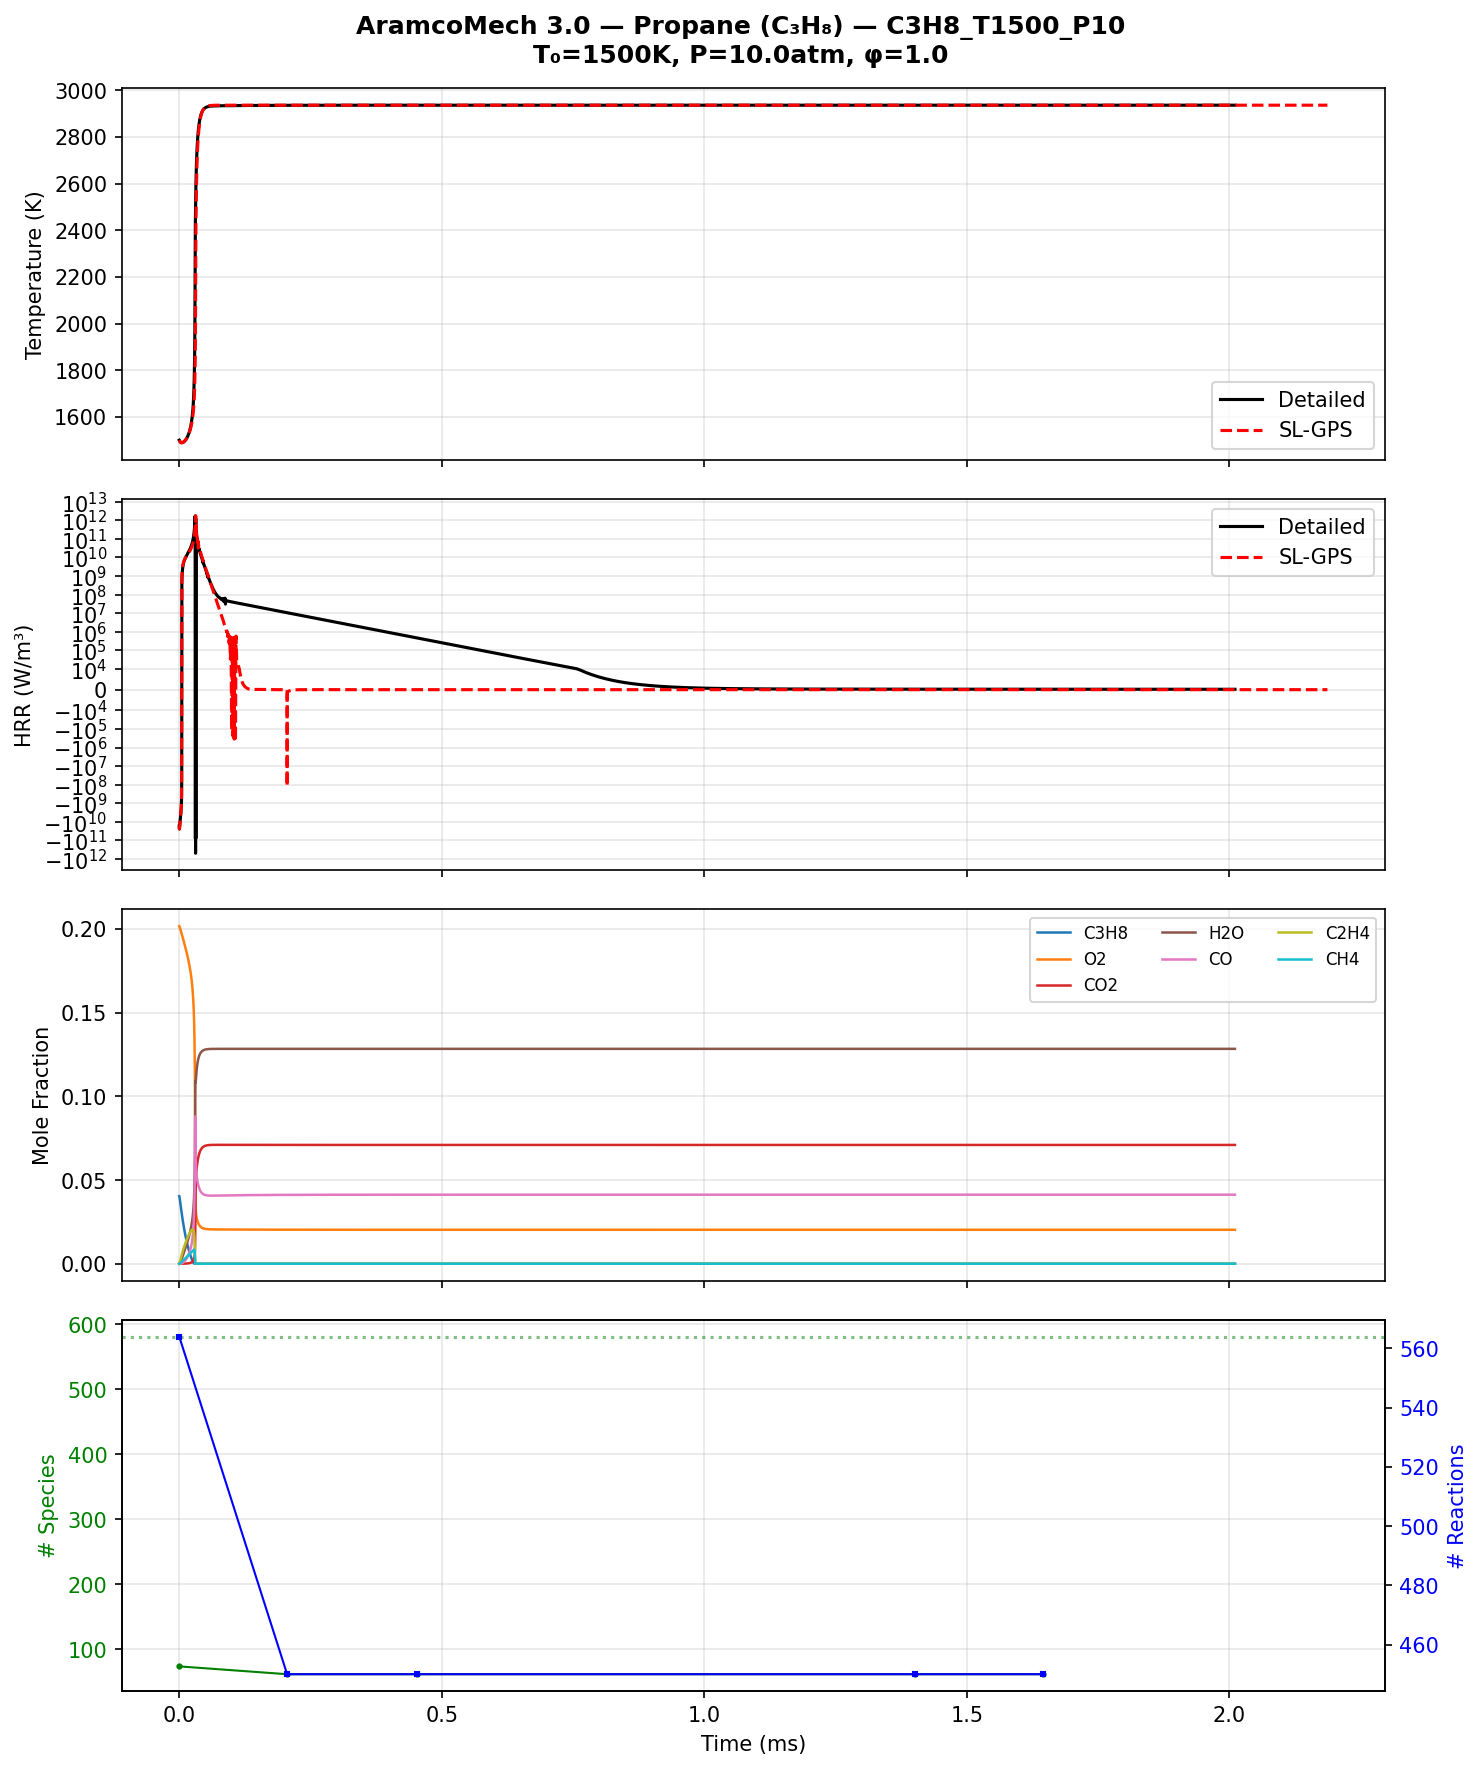
\includegraphics[width=0.95\textwidth]{results/c3h8/C3H8_T1500_P10.png}
    \caption{C$_3$H$_8$ Case 4: $T_0=1500$~K, $P=10$~atm, $\phi=1.0$.}
    \label{fig:c3h8_case4}
\end{figure}

\subsection{Results --- Extended Cases}

These cases test robustness under more challenging conditions: low temperature / high pressure (NTC regime), fuel-rich, fuel-lean, and extreme high-$T$/high-$P$.

\begin{figure}[H]
    \centering
    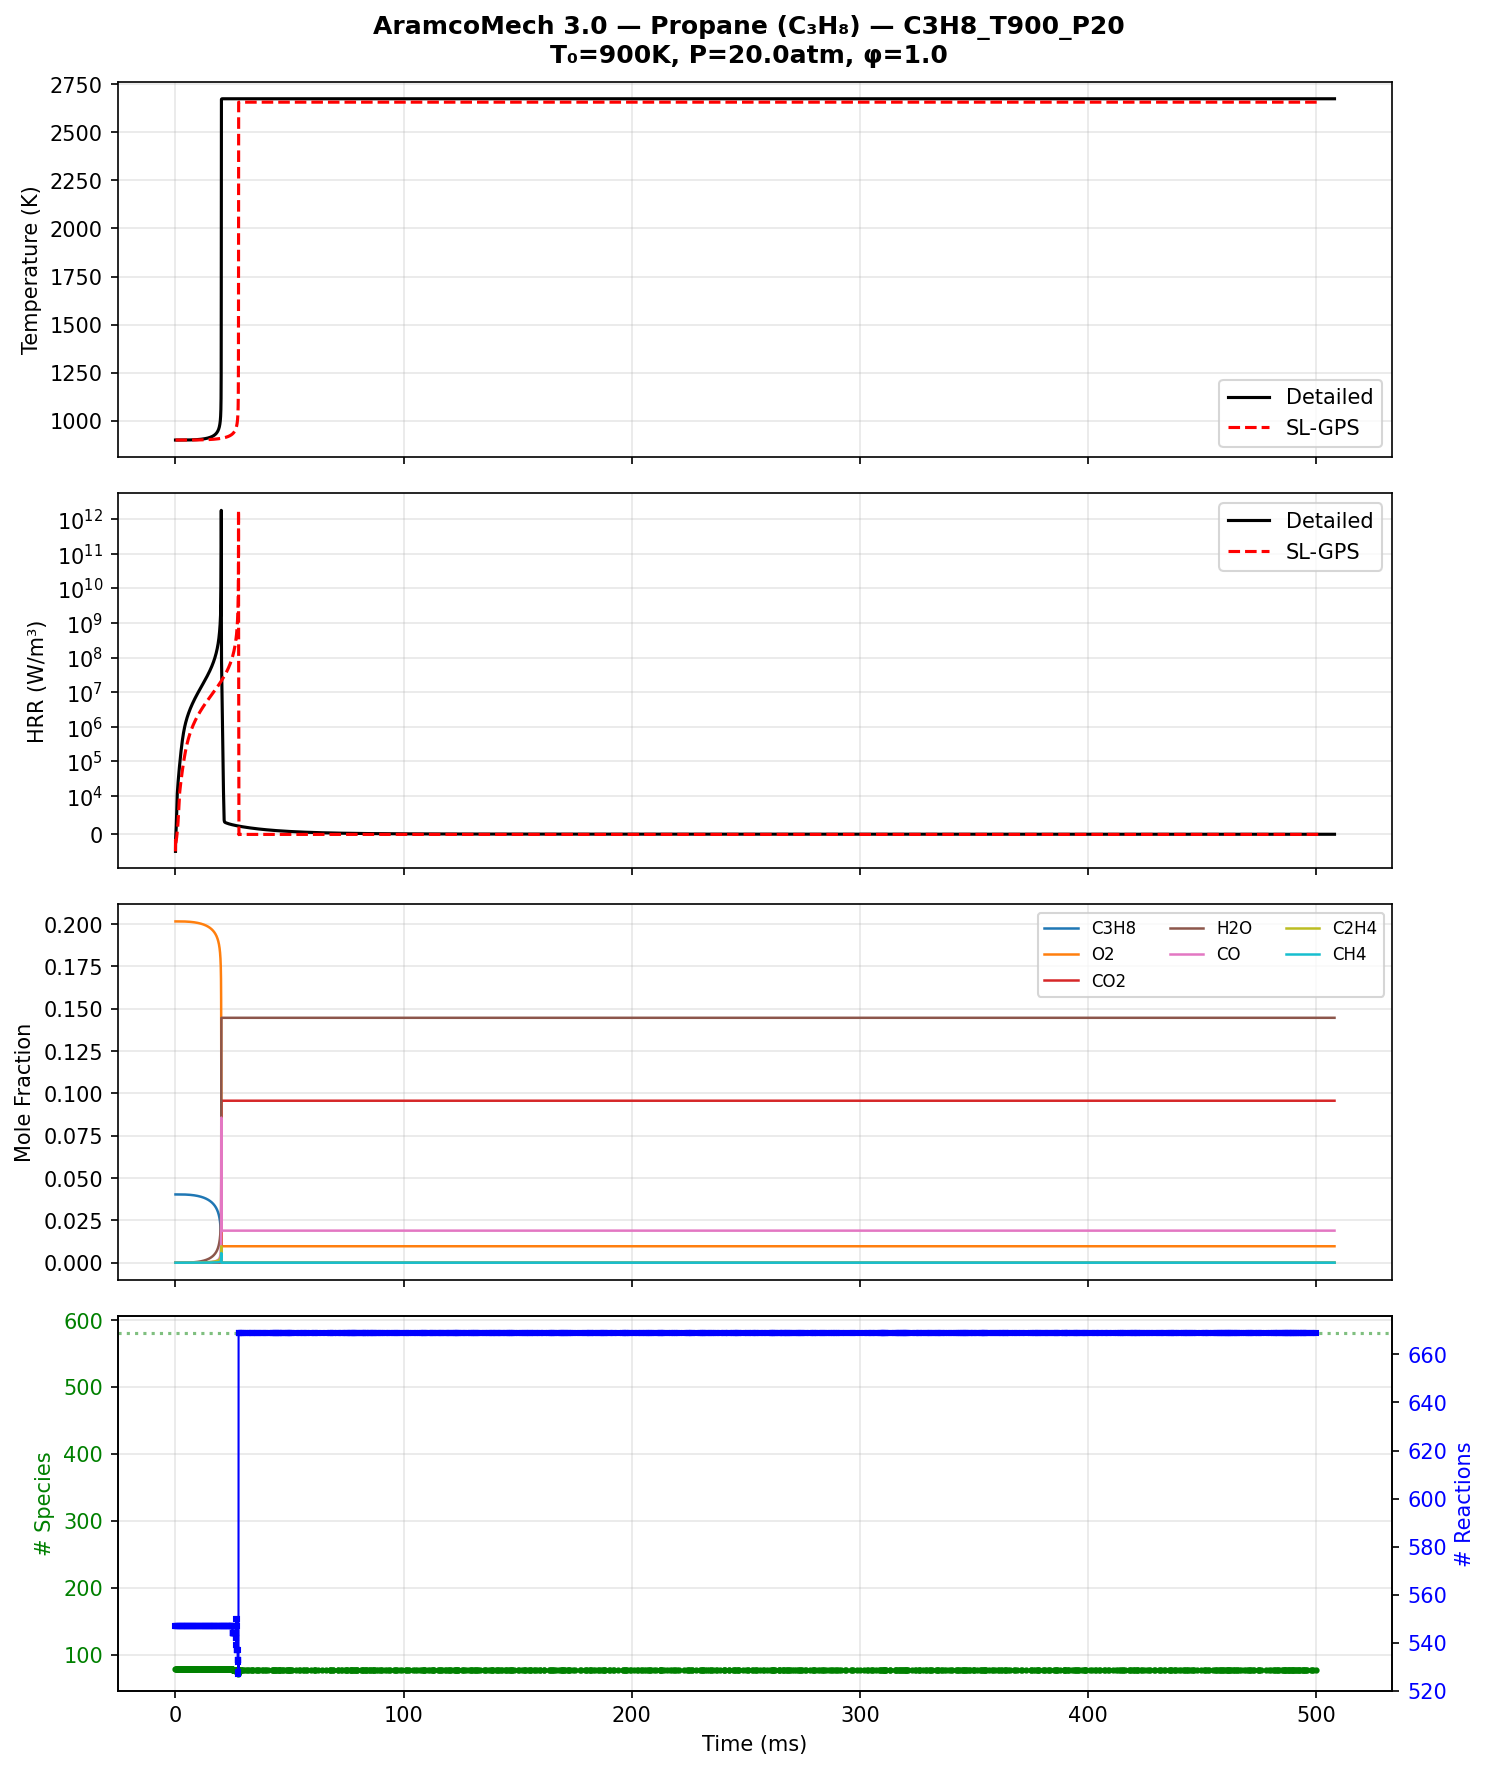
\includegraphics[width=0.95\textwidth]{results/c3h8/C3H8_T900_P20.png}
    \caption{C$_3$H$_8$ Case 5: $T_0=900$~K, $P=20$~atm, $\phi=1.0$. Low-temperature / high-pressure regime.}
    \label{fig:c3h8_case5}
\end{figure}

\begin{figure}[H]
    \centering
    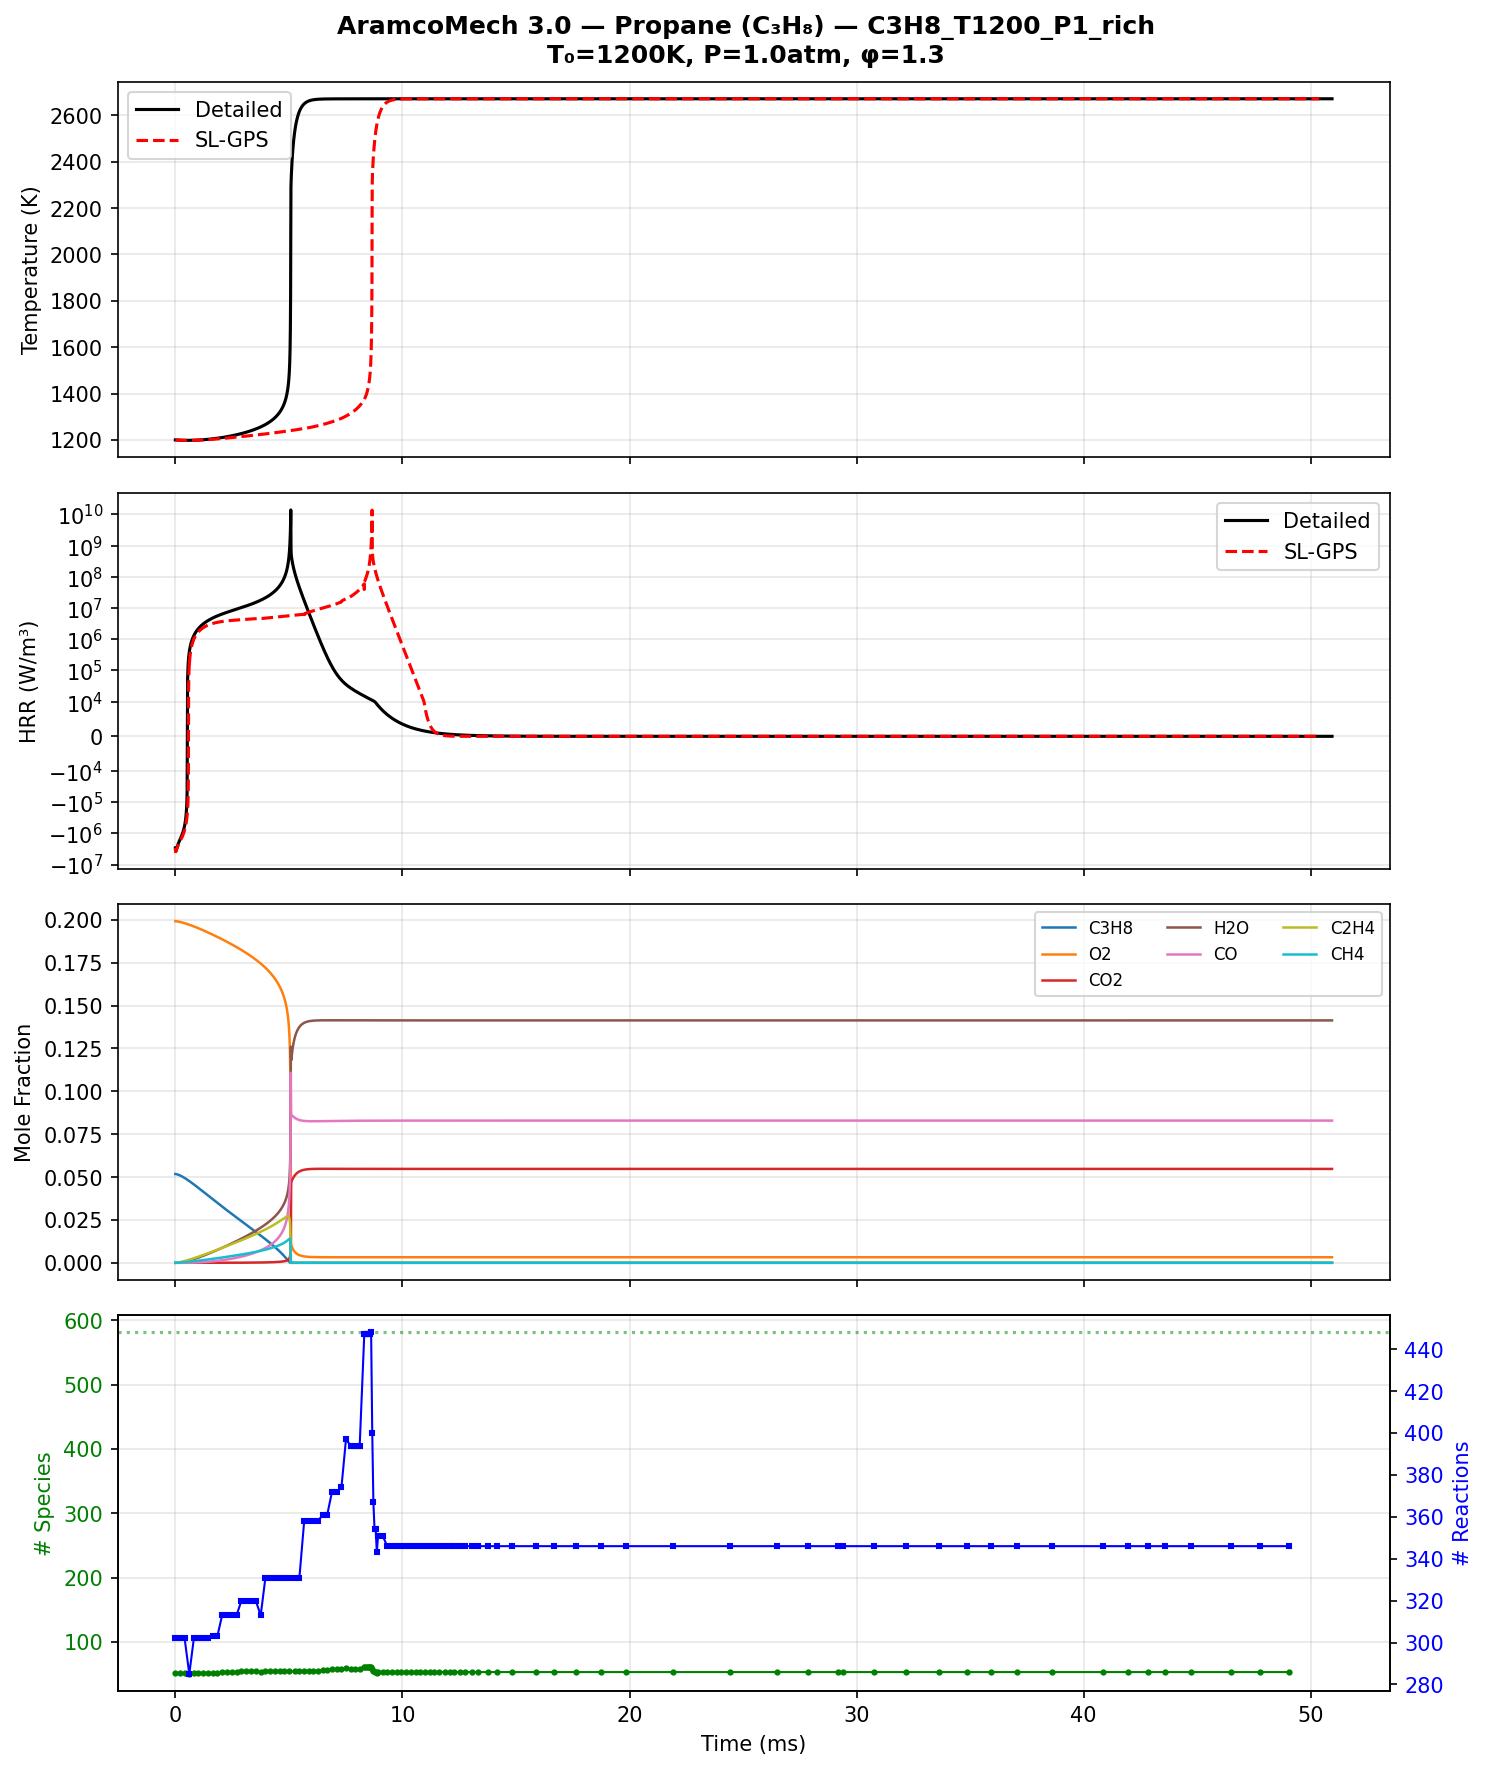
\includegraphics[width=0.95\textwidth]{results/c3h8/C3H8_T1200_P1_rich.png}
    \caption{C$_3$H$_8$ Case 6: $T_0=1200$~K, $P=1$~atm, $\phi=1.3$. Fuel-rich.}
    \label{fig:c3h8_case6}
\end{figure}

\begin{figure}[H]
    \centering
    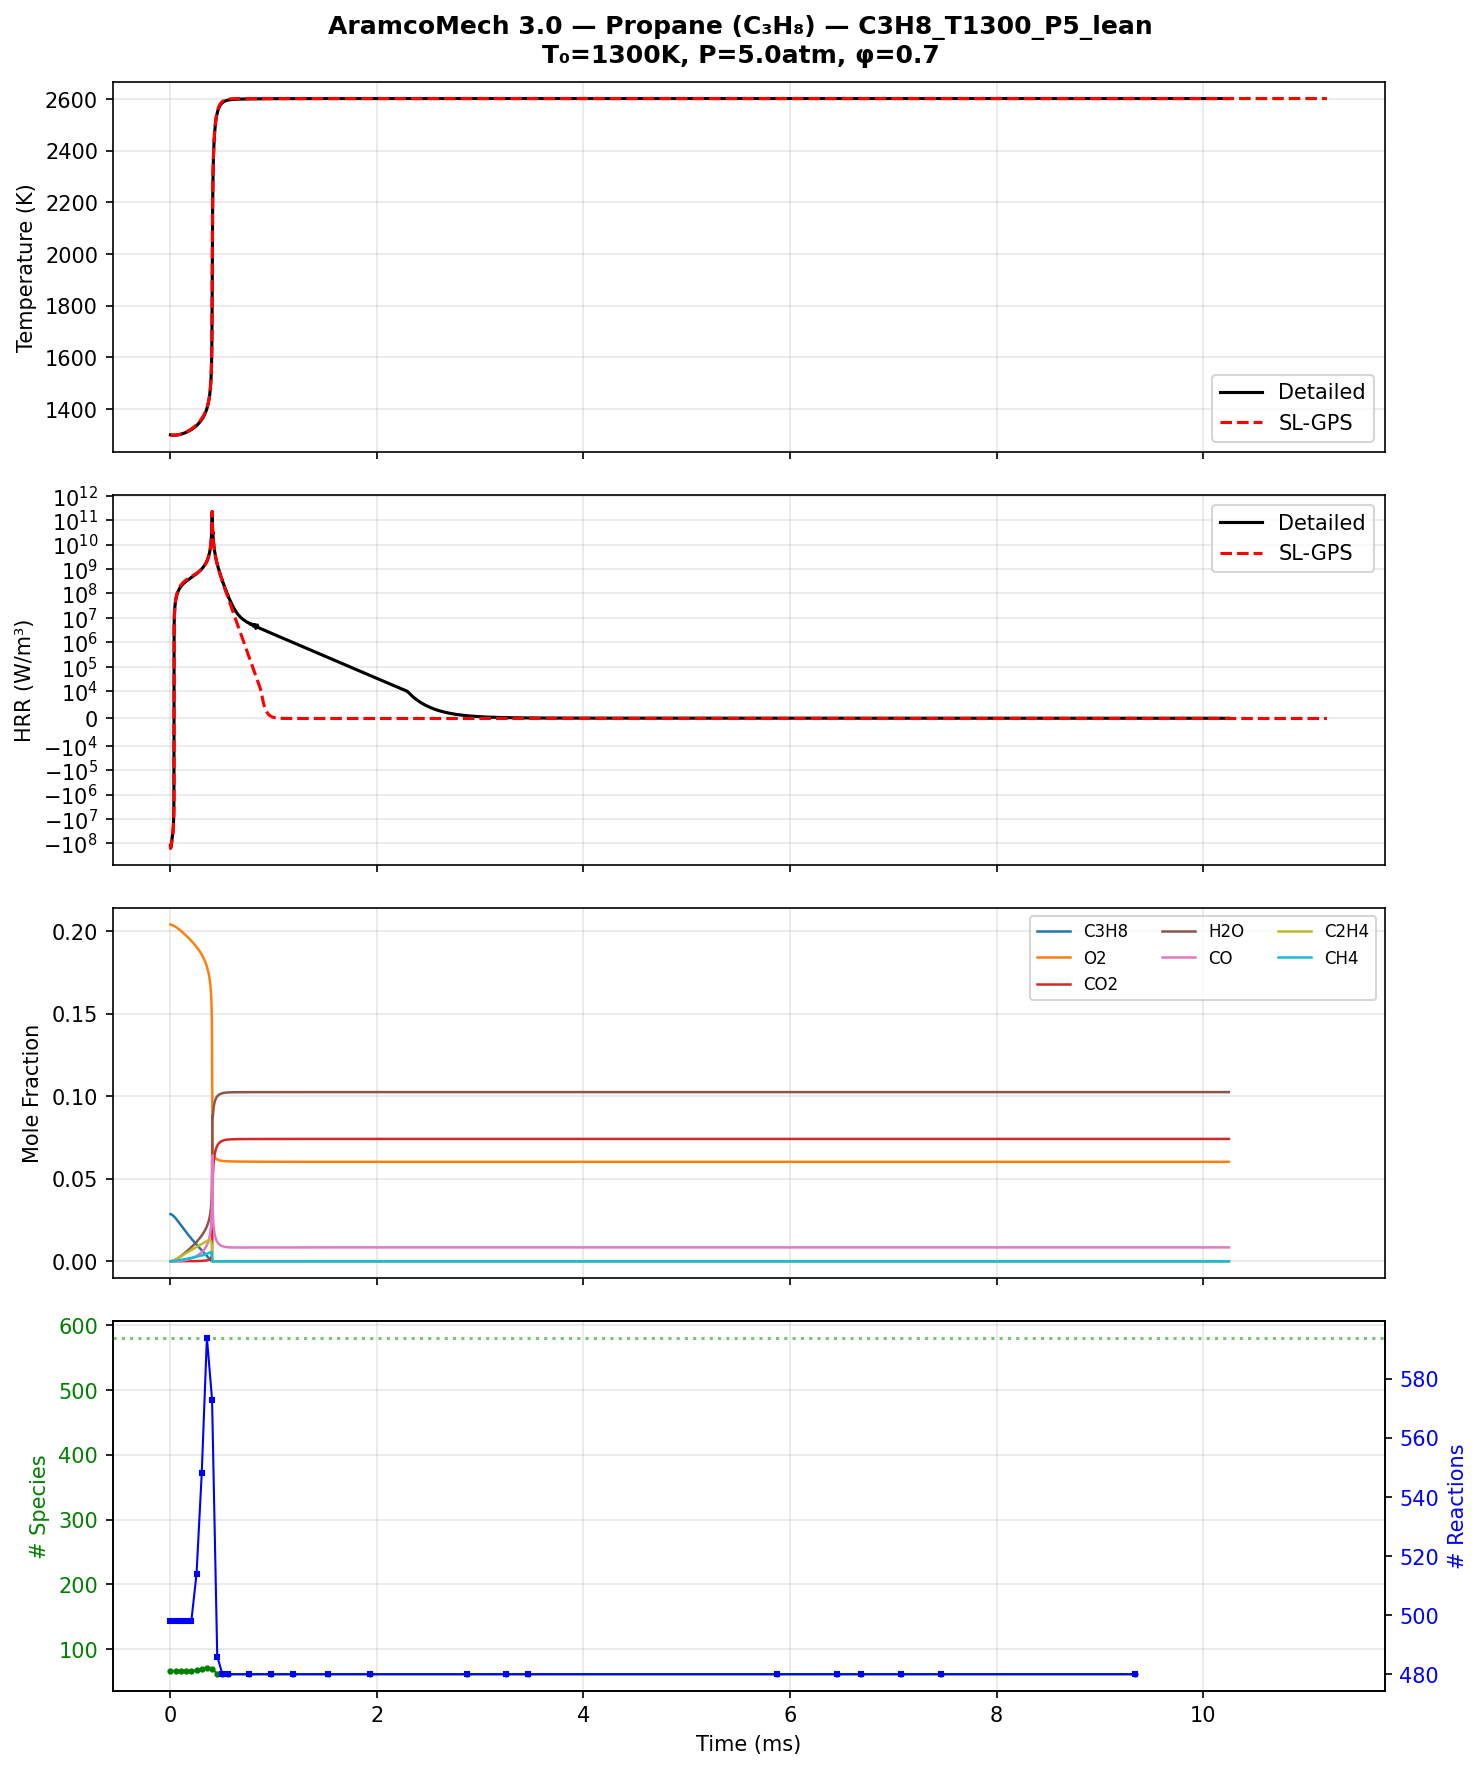
\includegraphics[width=0.95\textwidth]{results/c3h8/C3H8_T1300_P5_lean.png}
    \caption{C$_3$H$_8$ Case 7: $T_0=1300$~K, $P=5$~atm, $\phi=0.7$. Fuel-lean.}
    \label{fig:c3h8_case7}
\end{figure}

\begin{figure}[H]
    \centering
    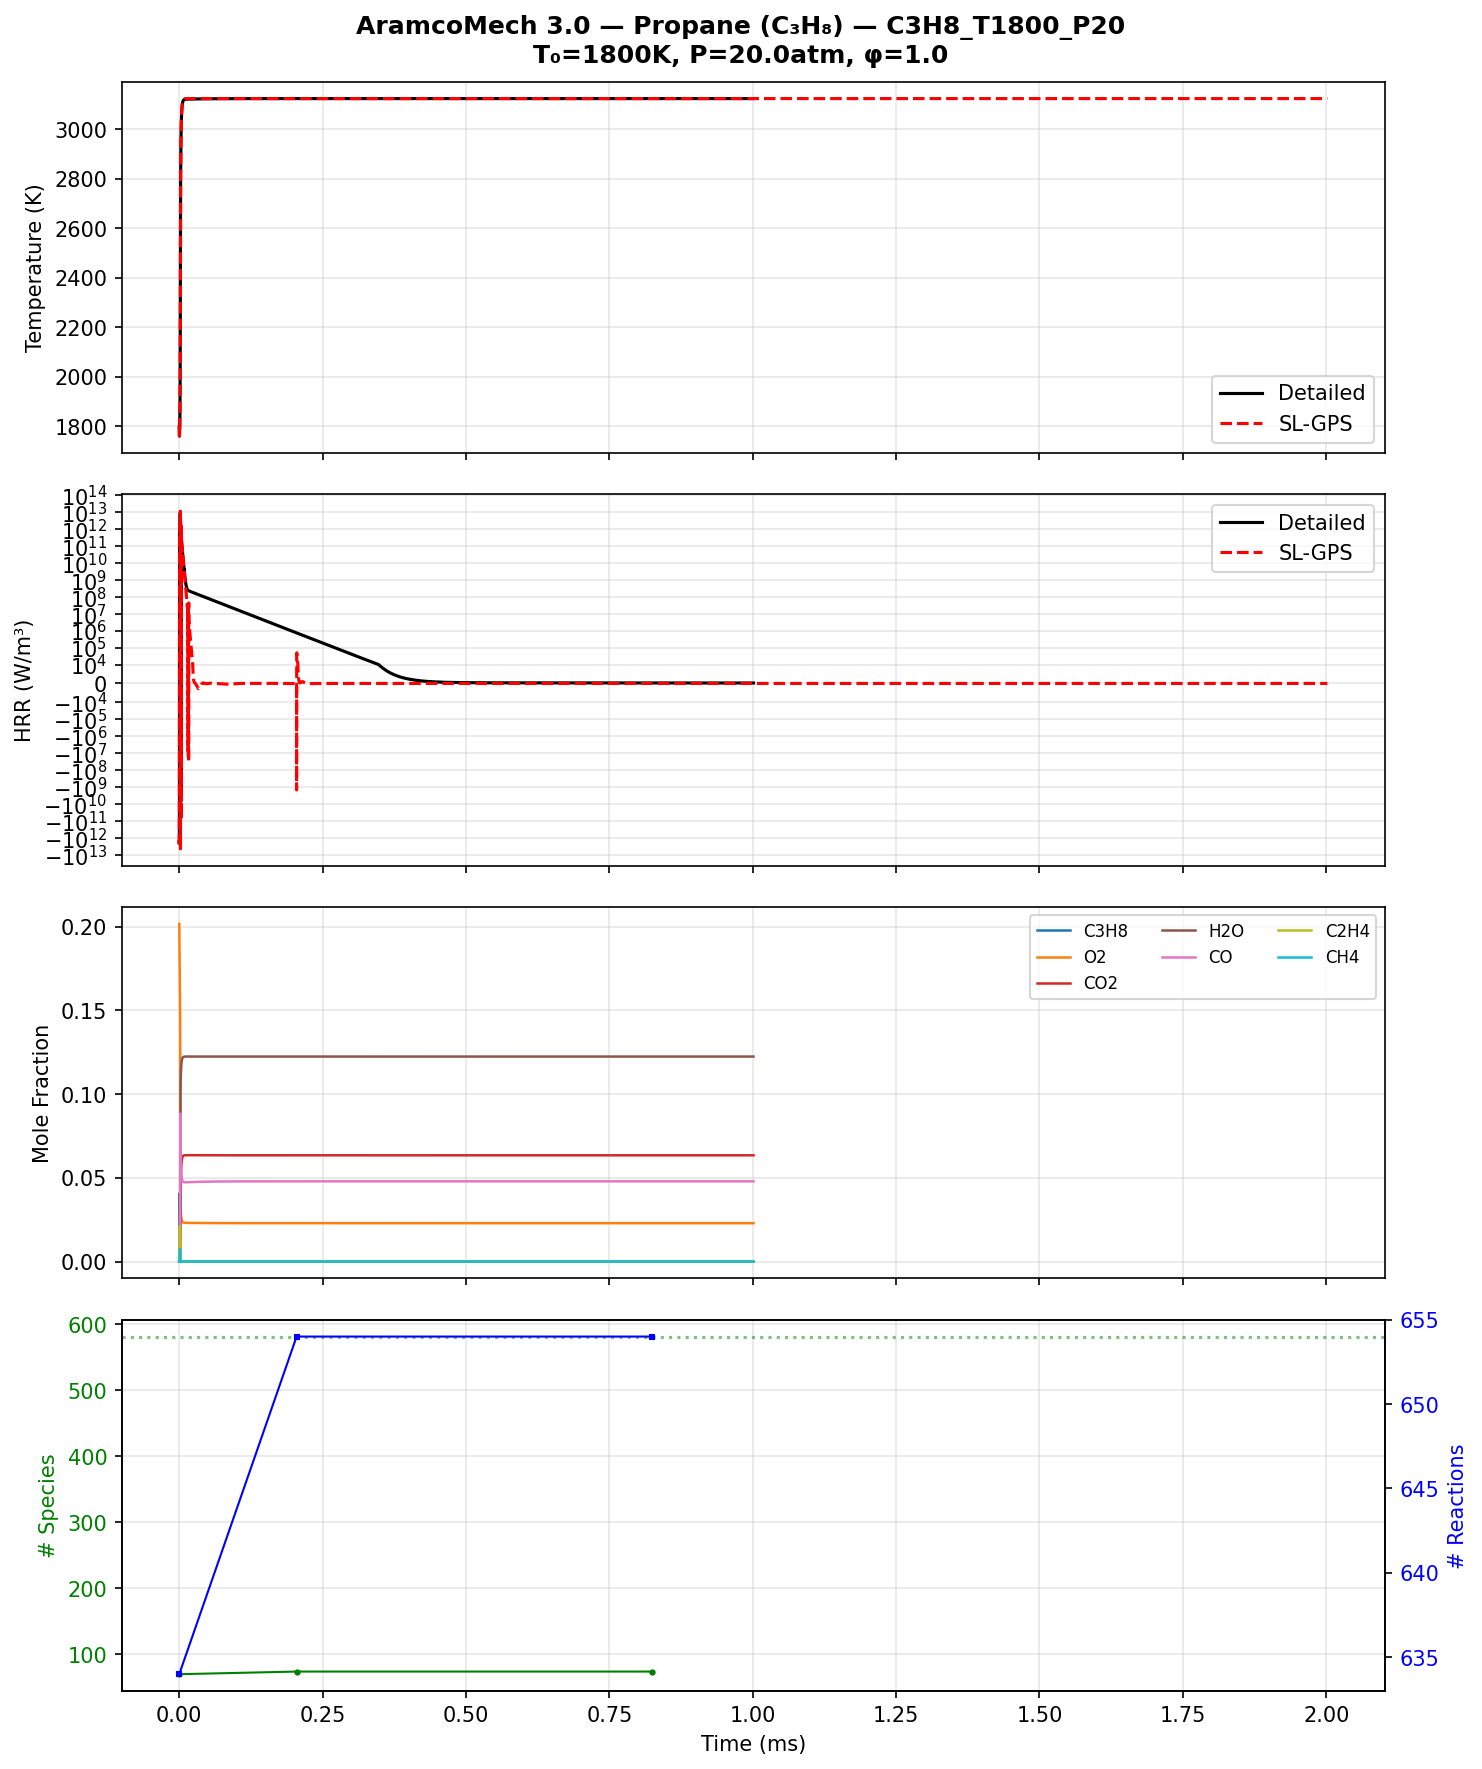
\includegraphics[width=0.95\textwidth]{results/c3h8/C3H8_T1800_P20.png}
    \caption{C$_3$H$_8$ Case 8: $T_0=1800$~K, $P=20$~atm, $\phi=1.0$. High-$T$ / high-$P$ (fast ignition).}
    \label{fig:c3h8_case8}
\end{figure}

\subsection{Summary and Timing}

\begin{figure}[H]
    \centering
    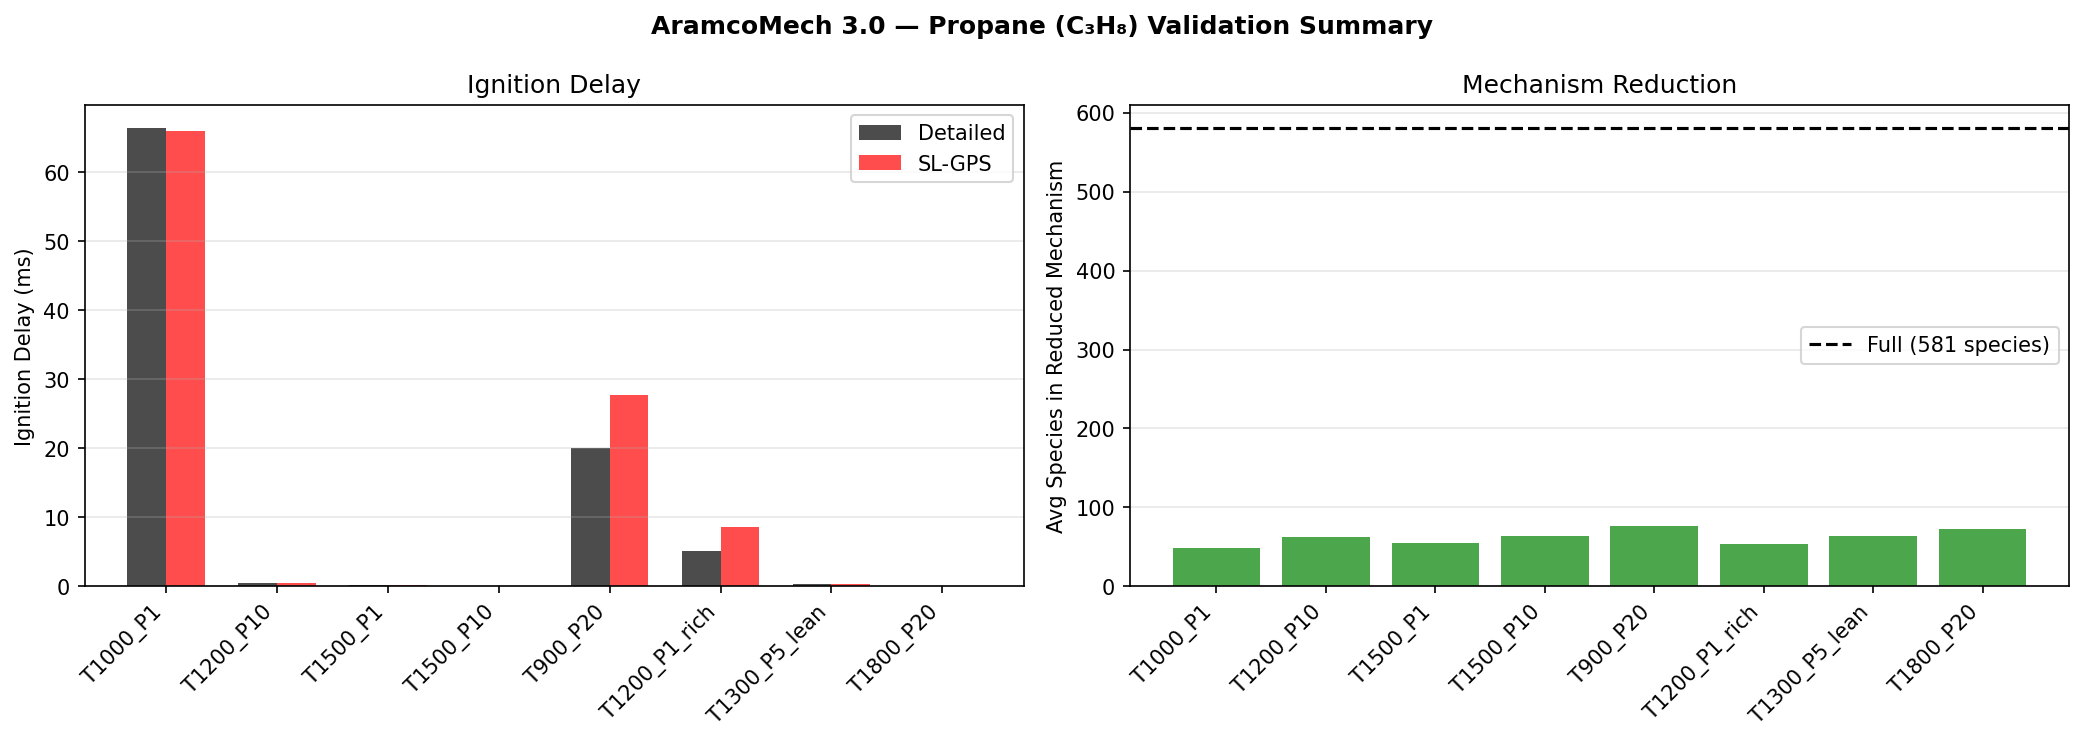
\includegraphics[width=0.95\textwidth]{results/c3h8/C3H8_summary.png}
    \caption{C$_3$H$_8$ summary. Left: ignition delay comparison. Right: average mechanism size (reduced vs.\ full 581 species).}
    \label{fig:c3h8_summary}
\end{figure}

\begin{table}[H]
\centering
\caption{C$_3$H$_8$ per-case timing.}
\label{tab:c3h8_timing}
\begin{tabular}{lcccc}
\toprule
\textbf{Case} & \textbf{Steps} & \textbf{Chemistry (s)} & \textbf{ANN (s)} & \textbf{Ratio} \\
\midrule
C3H8\_T1000\_P1 & 4429 & 0.80 & 21.1 & 26$\times$ \\
C3H8\_T1200\_P10 & 4635 & 0.57 & 2.1 & 3.7$\times$ \\
C3H8\_T1500\_P1 & 2945 & 0.38 & 1.5 & 4.0$\times$ \\
C3H8\_T1500\_P10 & 3773 & 0.44 & 0.30 & 0.7$\times$ \\
\midrule
C3H8\_T900\_P20 & 5800 & 2.09 & 52.0 & 25$\times$ \\
C3H8\_T1200\_P1\_rich & 4285 & 0.53 & 6.3 & 12$\times$ \\
C3H8\_T1300\_P5\_lean & 4138 & 0.49 & 1.4 & 2.9$\times$ \\
C3H8\_T1800\_P20 & 3262 & 0.37 & 0.20 & 0.5$\times$ \\
\bottomrule
\end{tabular}
\end{table}

\textbf{Total pipeline:} Data generation 23.1~min + Training 35.0~s + Validation (8 cases) 6.5~min.

% =============================================================================
% =============================================================================
\newpage
\section{Ethylene (C\texorpdfstring{$_2$}{2}H\texorpdfstring{$_4$}{4}) --- AramcoMech 3.0}
\label{sec:c2h4}
% =============================================================================
% =============================================================================

\subsection{Training Configuration}

\begin{table}[H]
\centering
\caption{C$_2$H$_4$ training configuration summary.}
\label{tab:c2h4_config}
\begin{tabular}{ll}
\toprule
\textbf{Parameter} & \textbf{Value} \\
\midrule
\multicolumn{2}{l}{\textit{Mechanism}} \\
\quad Mechanism & AramcoMech 3.0 \\
\quad Species / Reactions & 581 / 3037 \\
\midrule
\multicolumn{2}{l}{\textit{Data Generation}} \\
\quad Training cases & 15 (serial execution) \\
\quad Temperature range & 900--1900~K (uniform) \\
\quad Pressure range & 1--20~atm (log-uniform) \\
\quad Equivalence ratio $\phi$ & 0.6--1.5 (uniform) \\
\quad GPS $\alpha$ & 0.001 \\
\quad Total training samples & 757 \\
\quad Data generation time & 1372.7~s (22.9~min) \\
\midrule
\multicolumn{2}{l}{\textit{Species Classification}} \\
\quad Always species & 15 \\
\quad Variable species (ANN outputs) & 123 \\
\quad Never species & 443 \\
\midrule
\multicolumn{2}{l}{\textit{ANN Training}} \\
\quad Input features & $T$, $P$ + 14 species mole fractions \\
\quad Architecture & 2 hidden layers $\times$ 32 neurons \\
\quad Ensemble size & 8 parallel trainings \\
\quad Max epochs / Early stopping & 200 / patience 30 \\
\quad Actual epochs (best model) & 62 (early stopped) \\
\quad Training time & 28.4~s \\
\bottomrule
\end{tabular}
\end{table}

\textbf{Input species (ANN features):} C$_2$H$_4$, O$_2$, H$_2$O, CO$_2$, CO, OH, H, H$_2$, CH$_4$, C$_2$H$_2$, C$_2$H$_6$, CH$_2$O, HO$_2$, CH$_3$

\subsection{Validation Cases}

\begin{table}[H]
\centering
\caption{C$_2$H$_4$ validation conditions (4 baseline + 4 extended).}
\label{tab:c2h4_cases}
\begin{tabular}{lcccc}
\toprule
\textbf{Case} & \textbf{$T_0$ (K)} & \textbf{$P$ (atm)} & \textbf{$\phi$} & \textbf{$t_{\text{end}}$ (s)} \\
\midrule
C2H4\_T1000\_P1 & 1000 & 1 & 1.0 & 0.1 \\
C2H4\_T1200\_P10 & 1200 & 10 & 1.0 & 0.01 \\
C2H4\_T1500\_P1 & 1500 & 1 & 1.0 & 0.003 \\
C2H4\_T1500\_P10 & 1500 & 10 & 1.0 & 0.001 \\
\midrule
\multicolumn{5}{c}{\textit{Extended cases (difficult conditions)}} \\
\midrule
C2H4\_T900\_P20 & 900 & 20 & 1.0 & 0.5 \\
C2H4\_T1100\_P1\_rich & 1100 & 1 & 1.4 & 0.1 \\
C2H4\_T1300\_P5\_lean & 1300 & 5 & 0.7 & 0.005 \\
C2H4\_T1800\_P20 & 1800 & 20 & 1.0 & 0.0005 \\
\bottomrule
\end{tabular}
\end{table}

\subsection{Results --- Baseline Cases}

\begin{figure}[H]
    \centering
    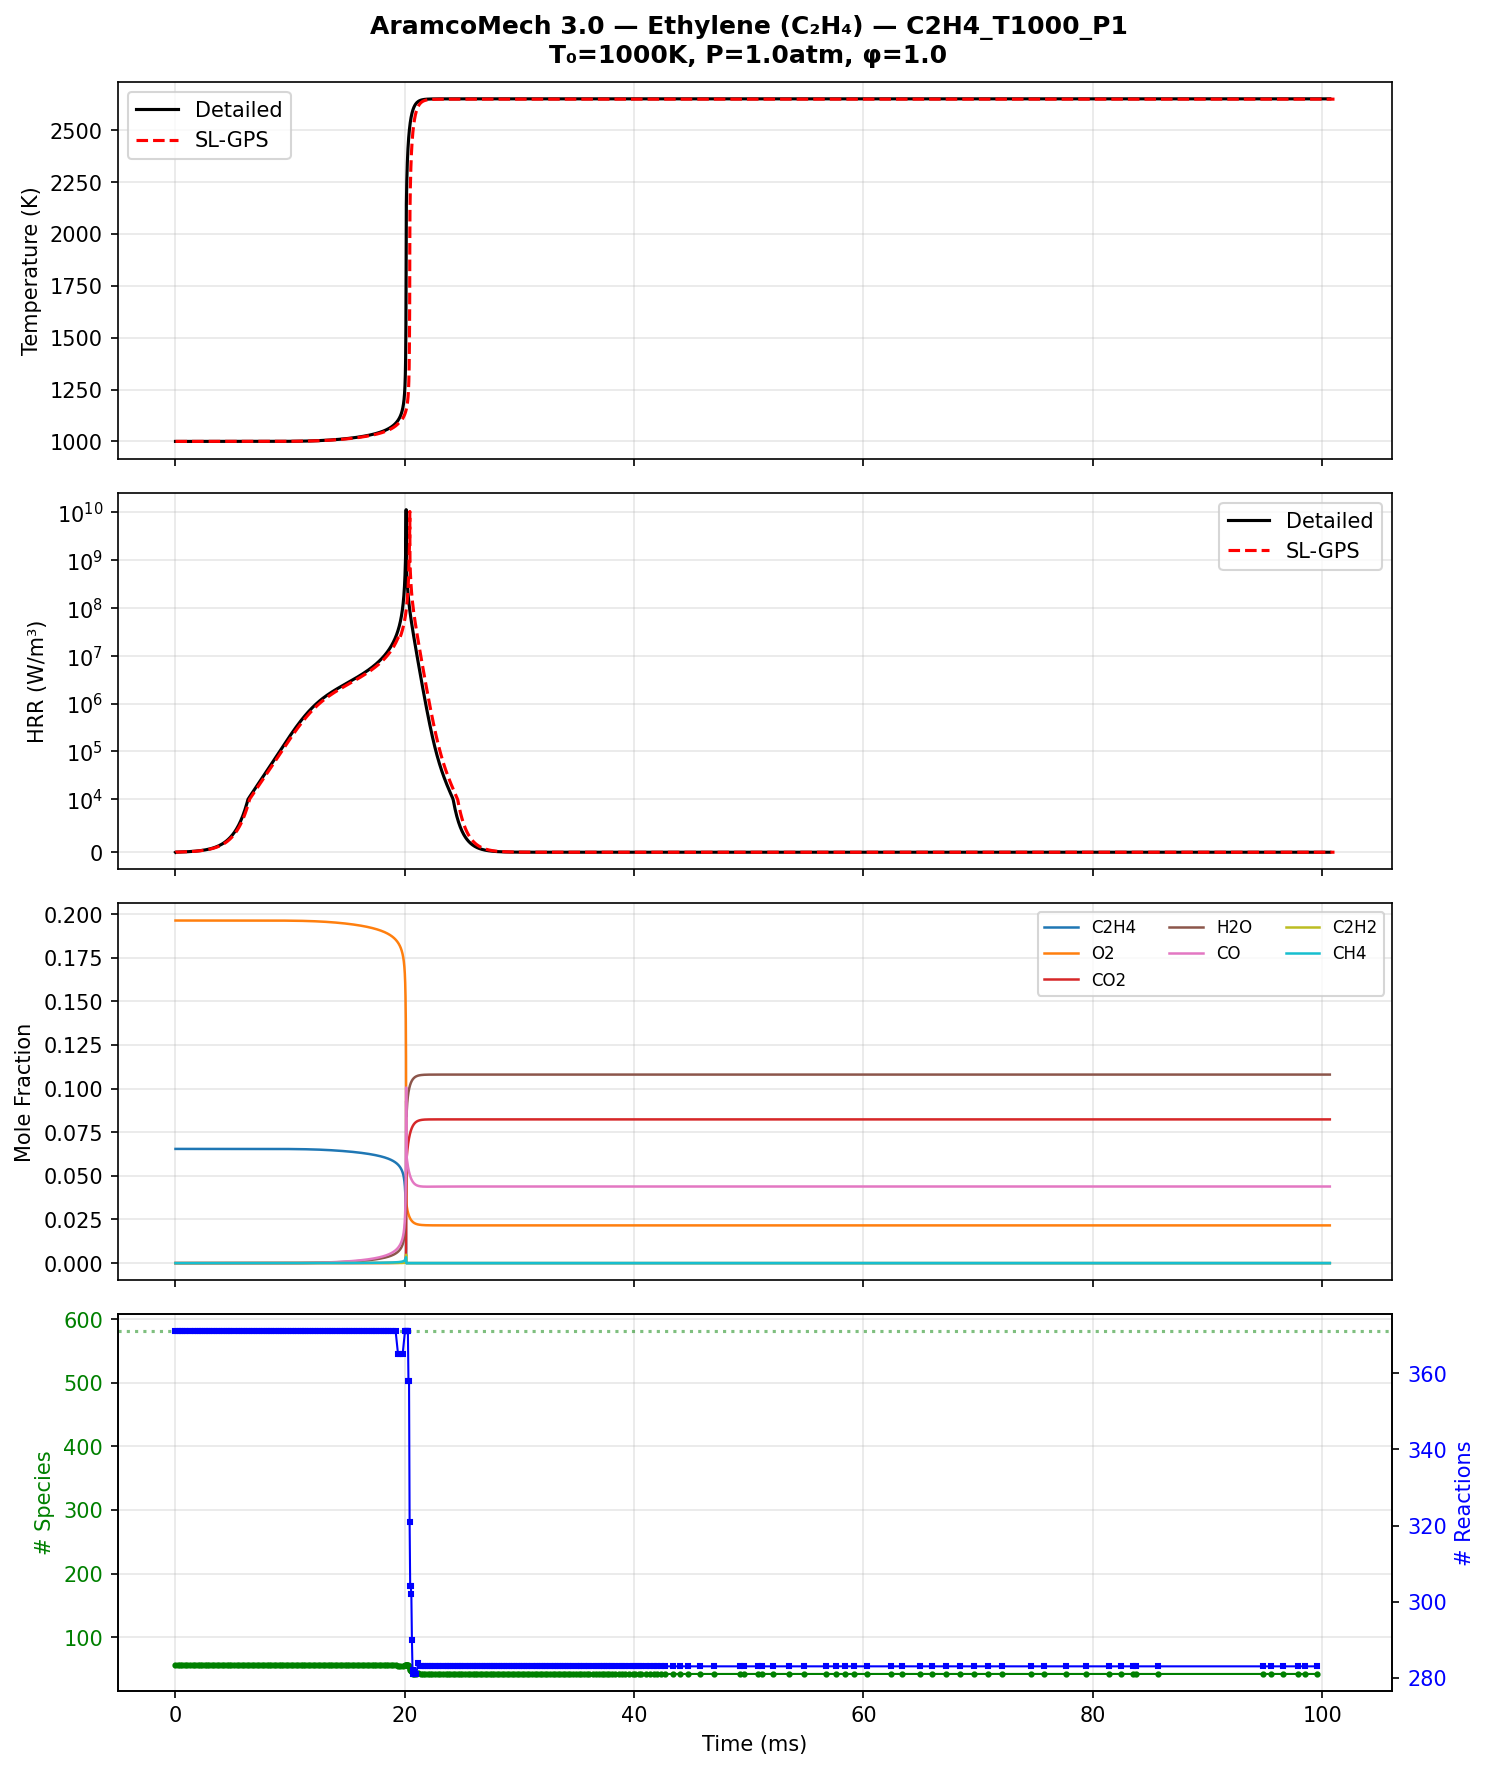
\includegraphics[width=0.95\textwidth]{results/c2h4/C2H4_T1000_P1.png}
    \caption{C$_2$H$_4$ Case 1: $T_0=1000$~K, $P=1$~atm, $\phi=1.0$.}
    \label{fig:c2h4_case1}
\end{figure}

\begin{figure}[H]
    \centering
    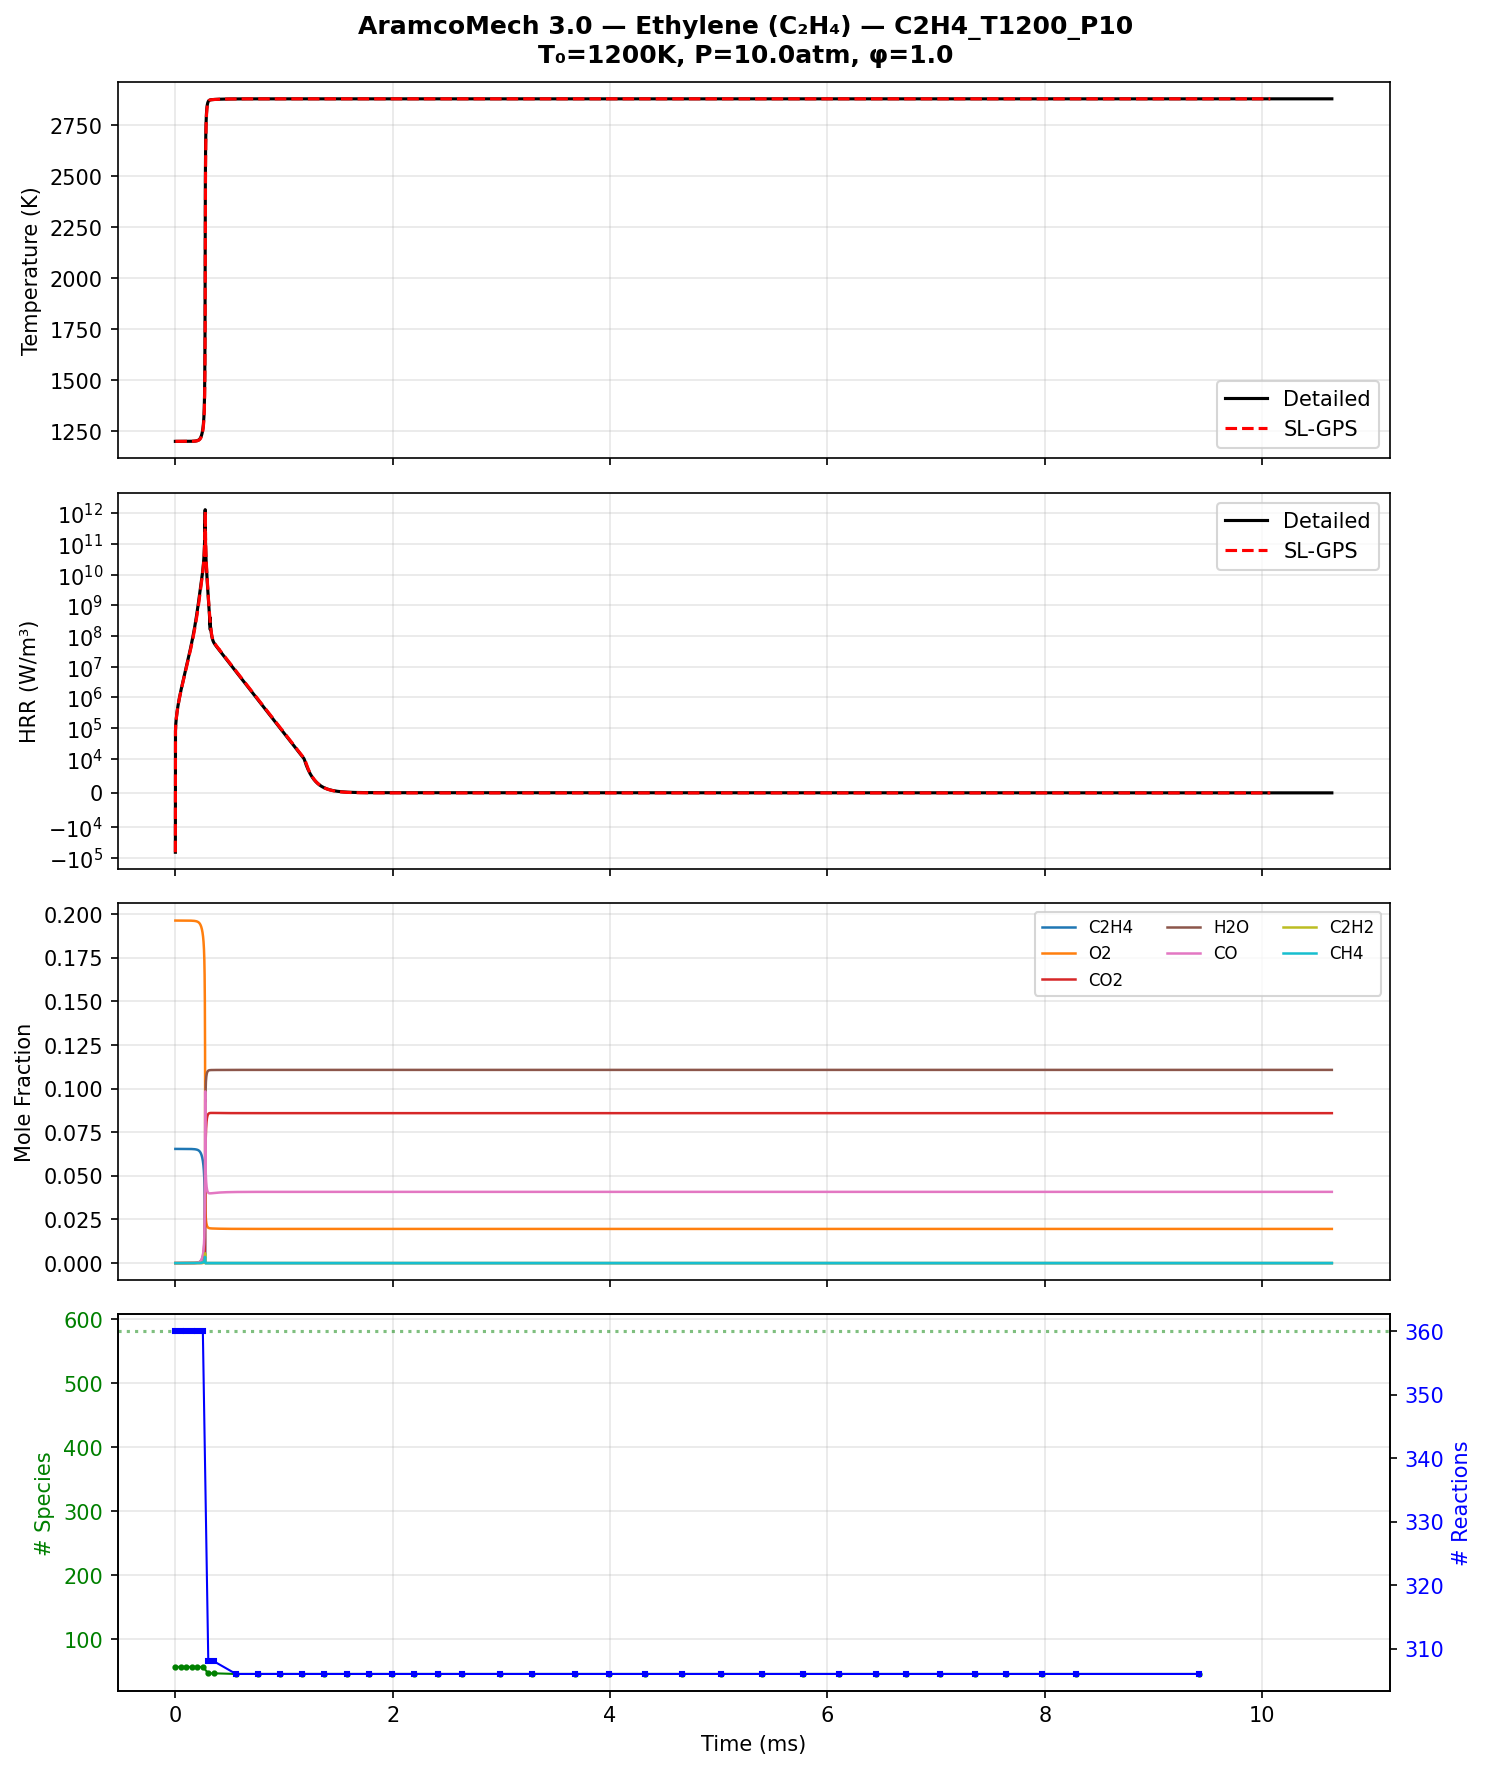
\includegraphics[width=0.95\textwidth]{results/c2h4/C2H4_T1200_P10.png}
    \caption{C$_2$H$_4$ Case 2: $T_0=1200$~K, $P=10$~atm, $\phi=1.0$.}
    \label{fig:c2h4_case2}
\end{figure}

\begin{figure}[H]
    \centering
    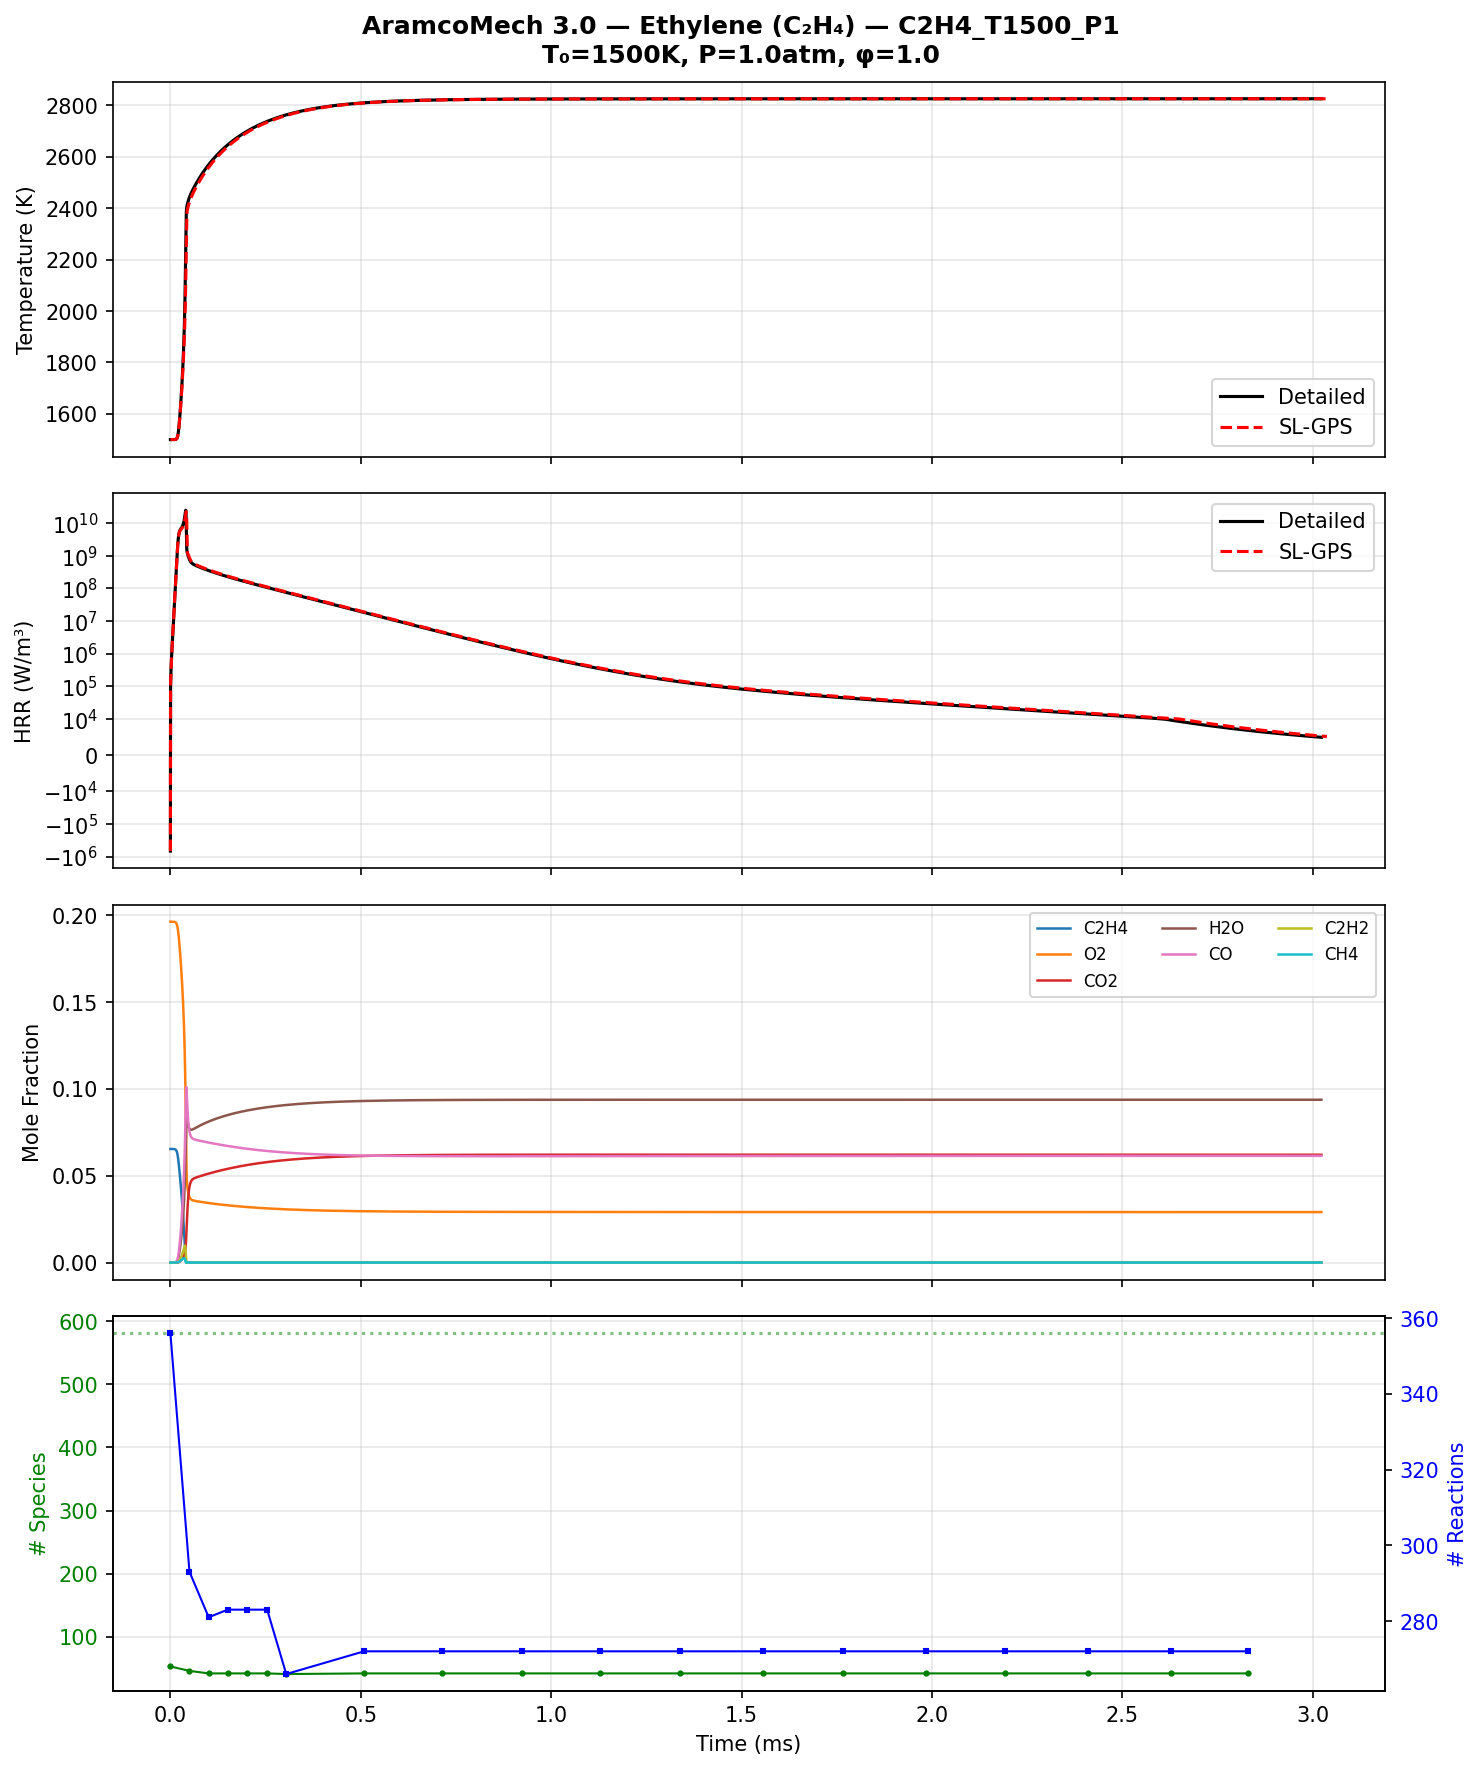
\includegraphics[width=0.95\textwidth]{results/c2h4/C2H4_T1500_P1.png}
    \caption{C$_2$H$_4$ Case 3: $T_0=1500$~K, $P=1$~atm, $\phi=1.0$.}
    \label{fig:c2h4_case3}
\end{figure}

\begin{figure}[H]
    \centering
    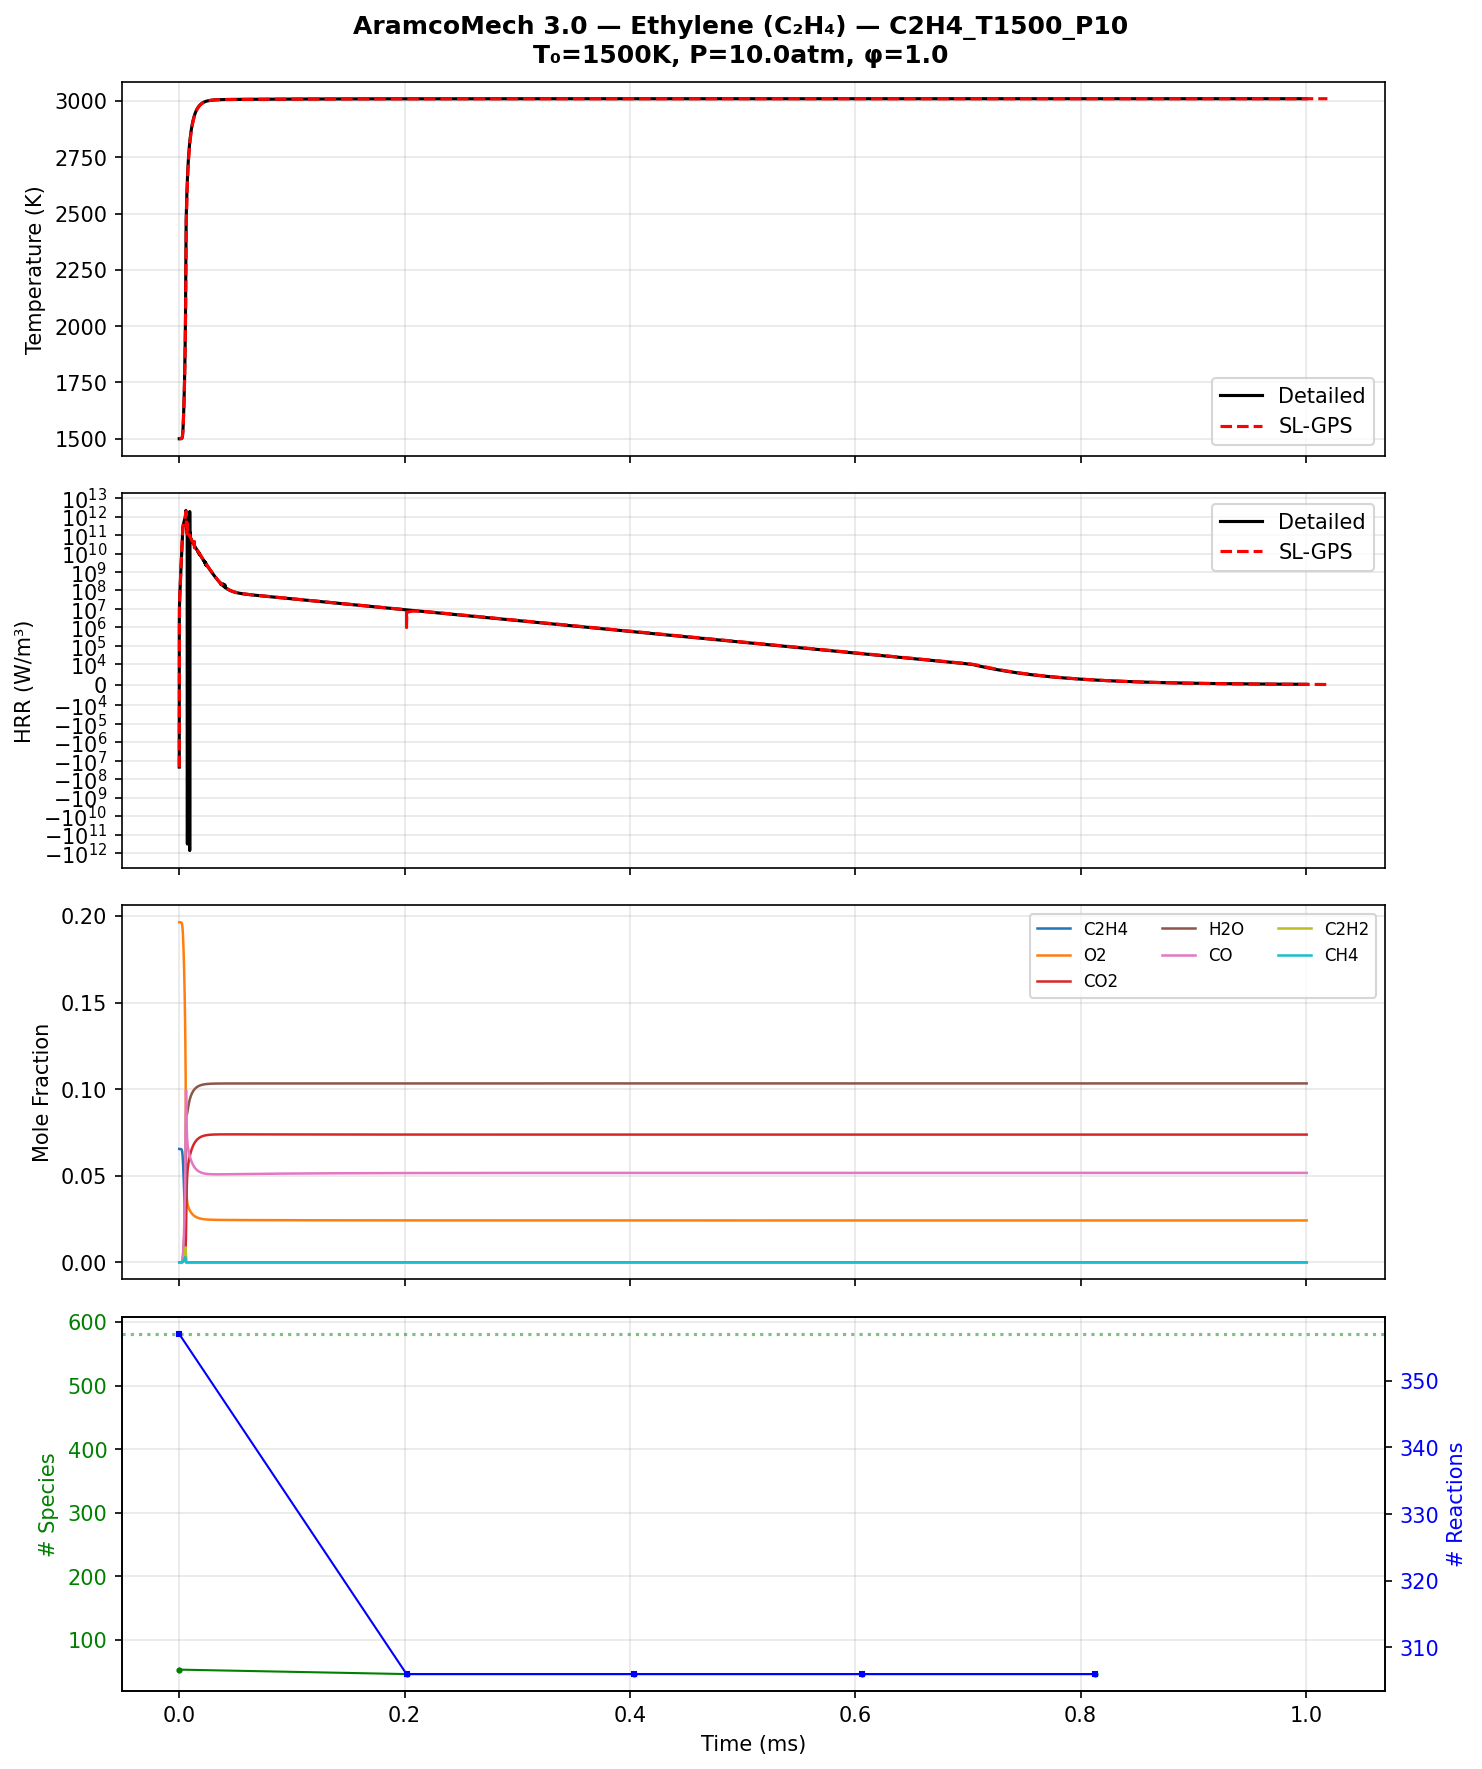
\includegraphics[width=0.95\textwidth]{results/c2h4/C2H4_T1500_P10.png}
    \caption{C$_2$H$_4$ Case 4: $T_0=1500$~K, $P=10$~atm, $\phi=1.0$.}
    \label{fig:c2h4_case4}
\end{figure}

\subsection{Results --- Extended Cases}

\begin{figure}[H]
    \centering
    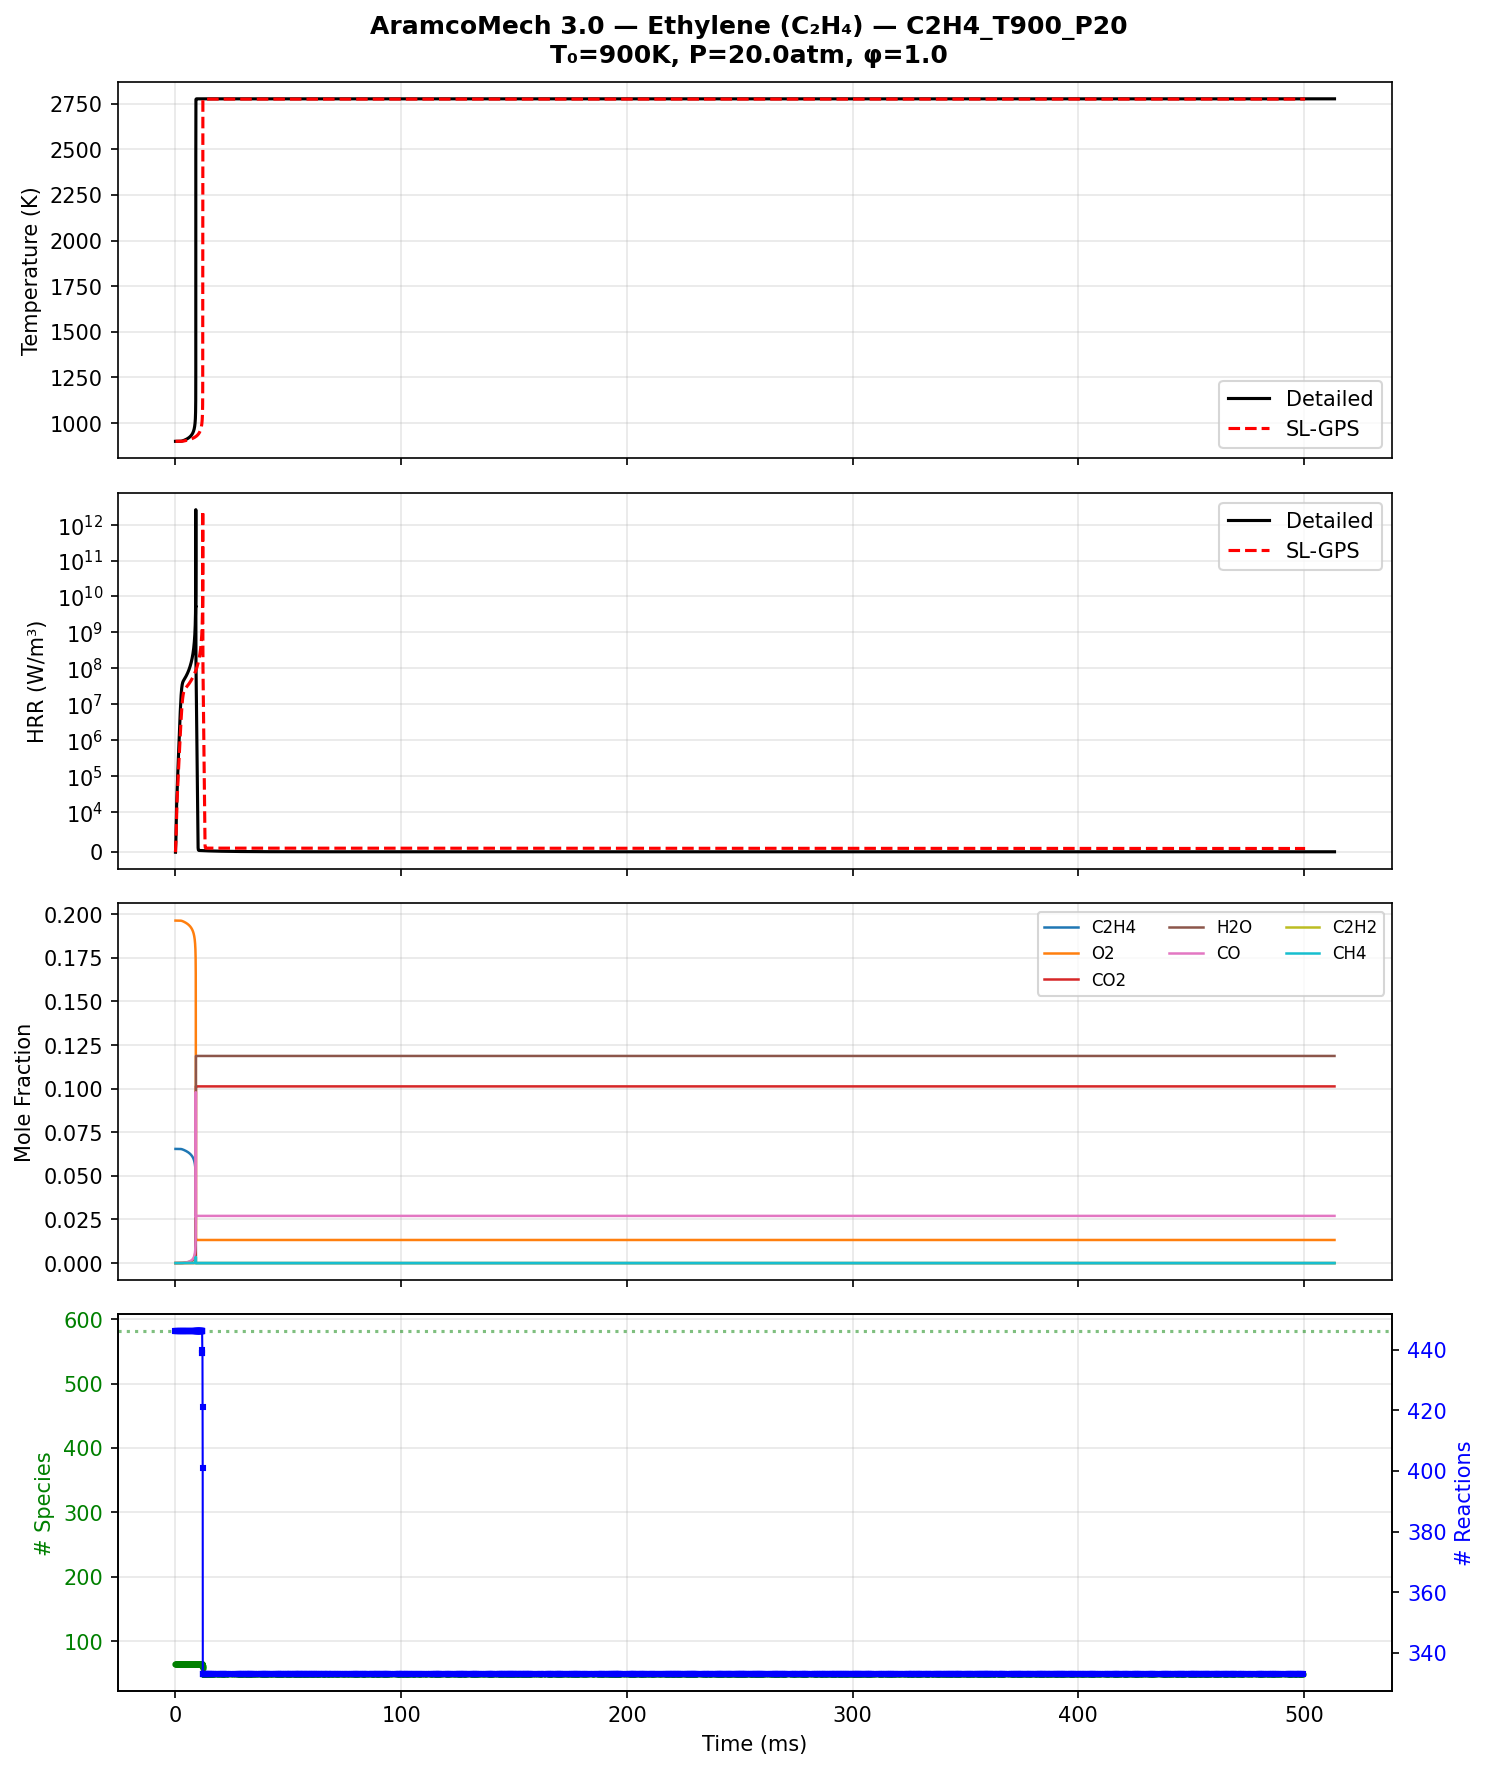
\includegraphics[width=0.95\textwidth]{results/c2h4/C2H4_T900_P20.png}
    \caption{C$_2$H$_4$ Case 5: $T_0=900$~K, $P=20$~atm, $\phi=1.0$. Low-temperature / high-pressure regime.}
    \label{fig:c2h4_case5}
\end{figure}

\begin{figure}[H]
    \centering
    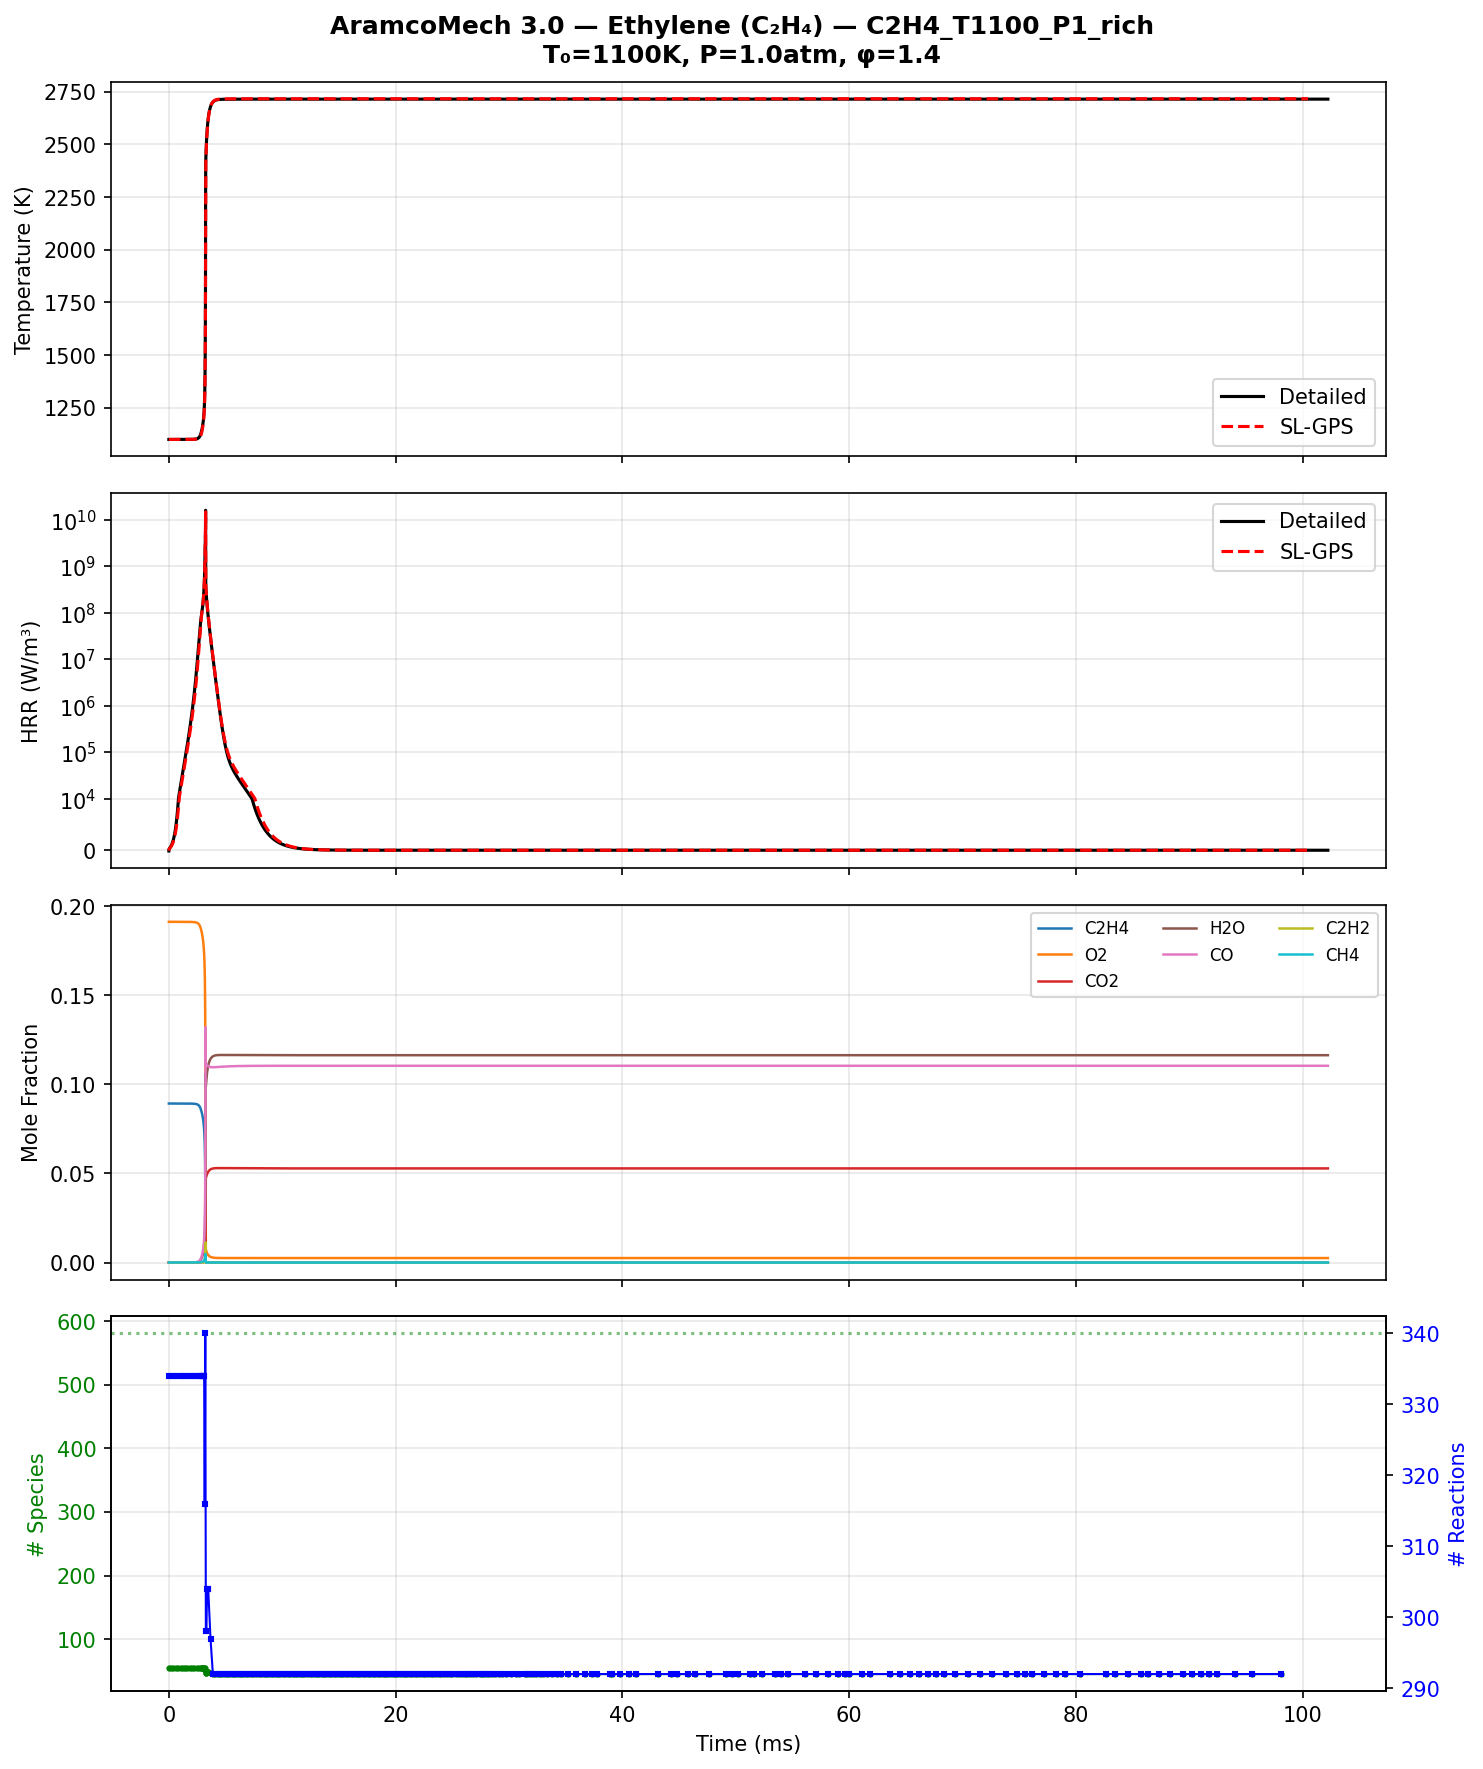
\includegraphics[width=0.95\textwidth]{results/c2h4/C2H4_T1100_P1_rich.png}
    \caption{C$_2$H$_4$ Case 6: $T_0=1100$~K, $P=1$~atm, $\phi=1.4$. Fuel-rich.}
    \label{fig:c2h4_case6}
\end{figure}

\begin{figure}[H]
    \centering
    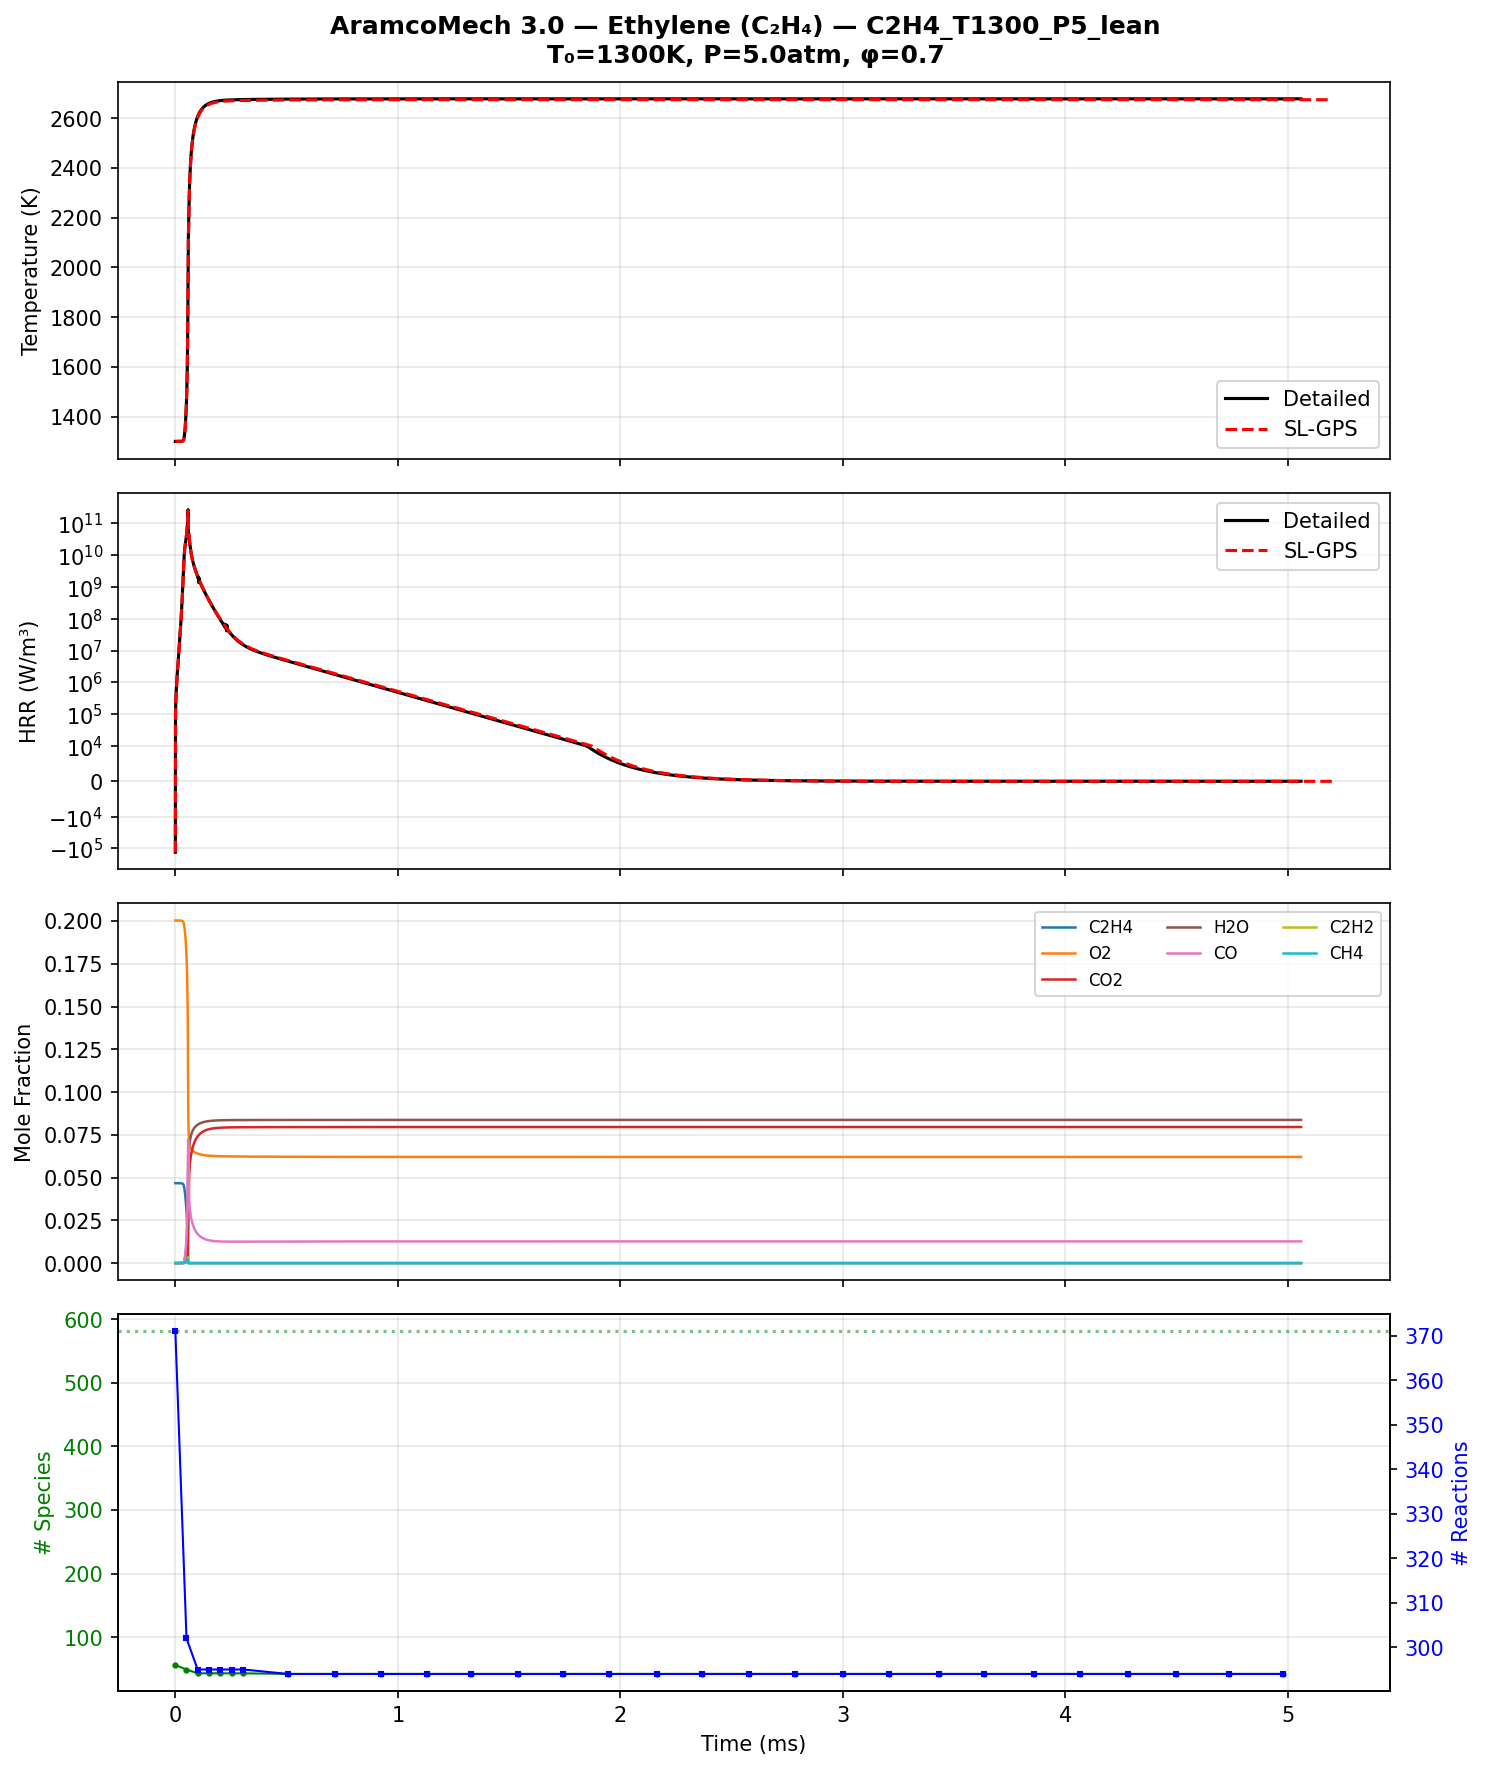
\includegraphics[width=0.95\textwidth]{results/c2h4/C2H4_T1300_P5_lean.png}
    \caption{C$_2$H$_4$ Case 7: $T_0=1300$~K, $P=5$~atm, $\phi=0.7$. Fuel-lean.}
    \label{fig:c2h4_case7}
\end{figure}

\begin{figure}[H]
    \centering
    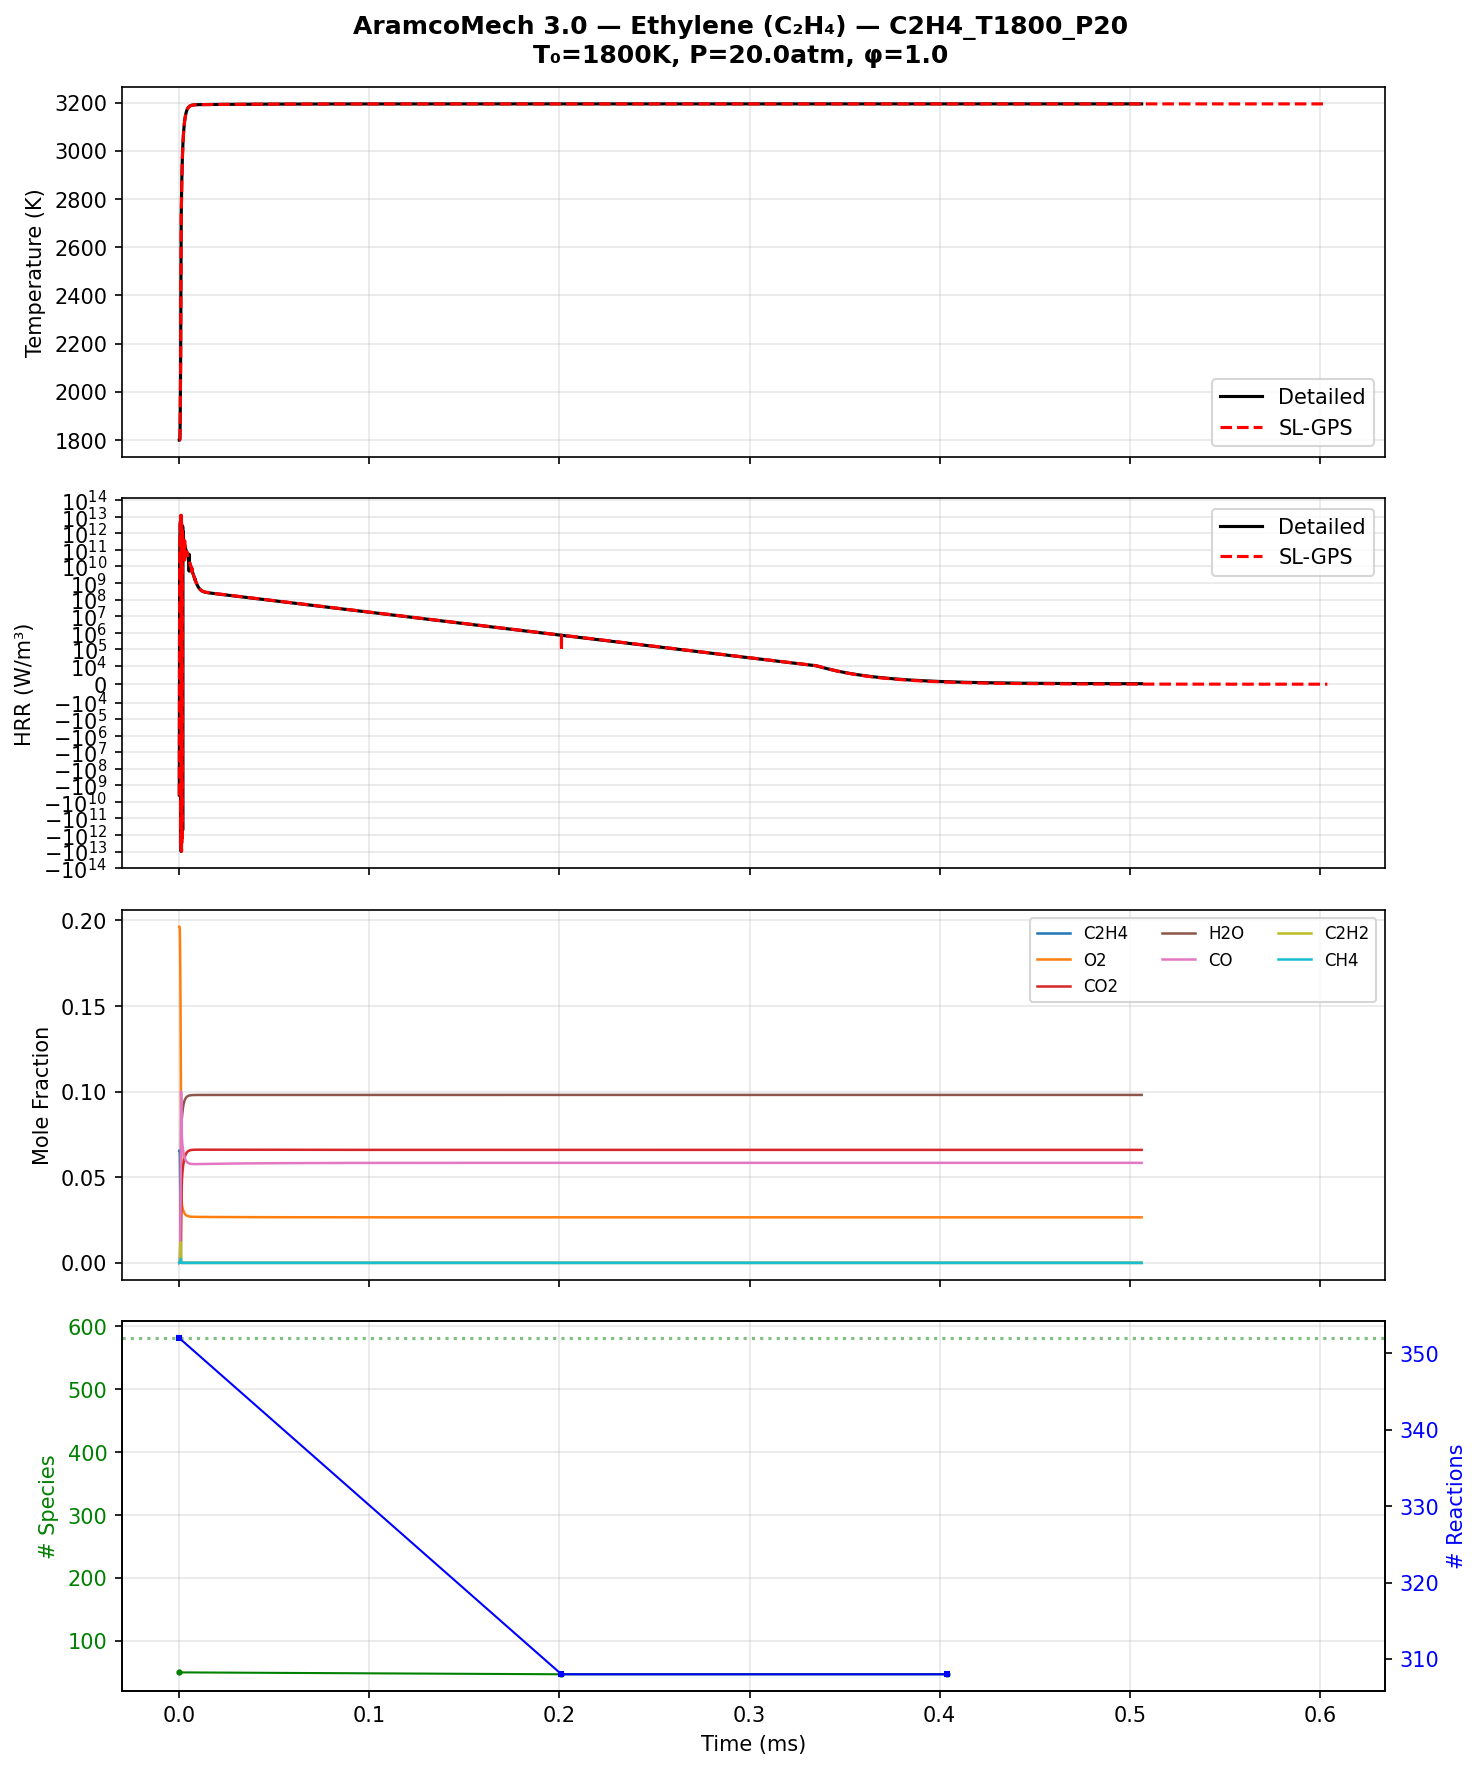
\includegraphics[width=0.95\textwidth]{results/c2h4/C2H4_T1800_P20.png}
    \caption{C$_2$H$_4$ Case 8: $T_0=1800$~K, $P=20$~atm, $\phi=1.0$. High-$T$ / high-$P$ (fast ignition).}
    \label{fig:c2h4_case8}
\end{figure}

\subsection{Summary and Timing}

\begin{figure}[H]
    \centering
    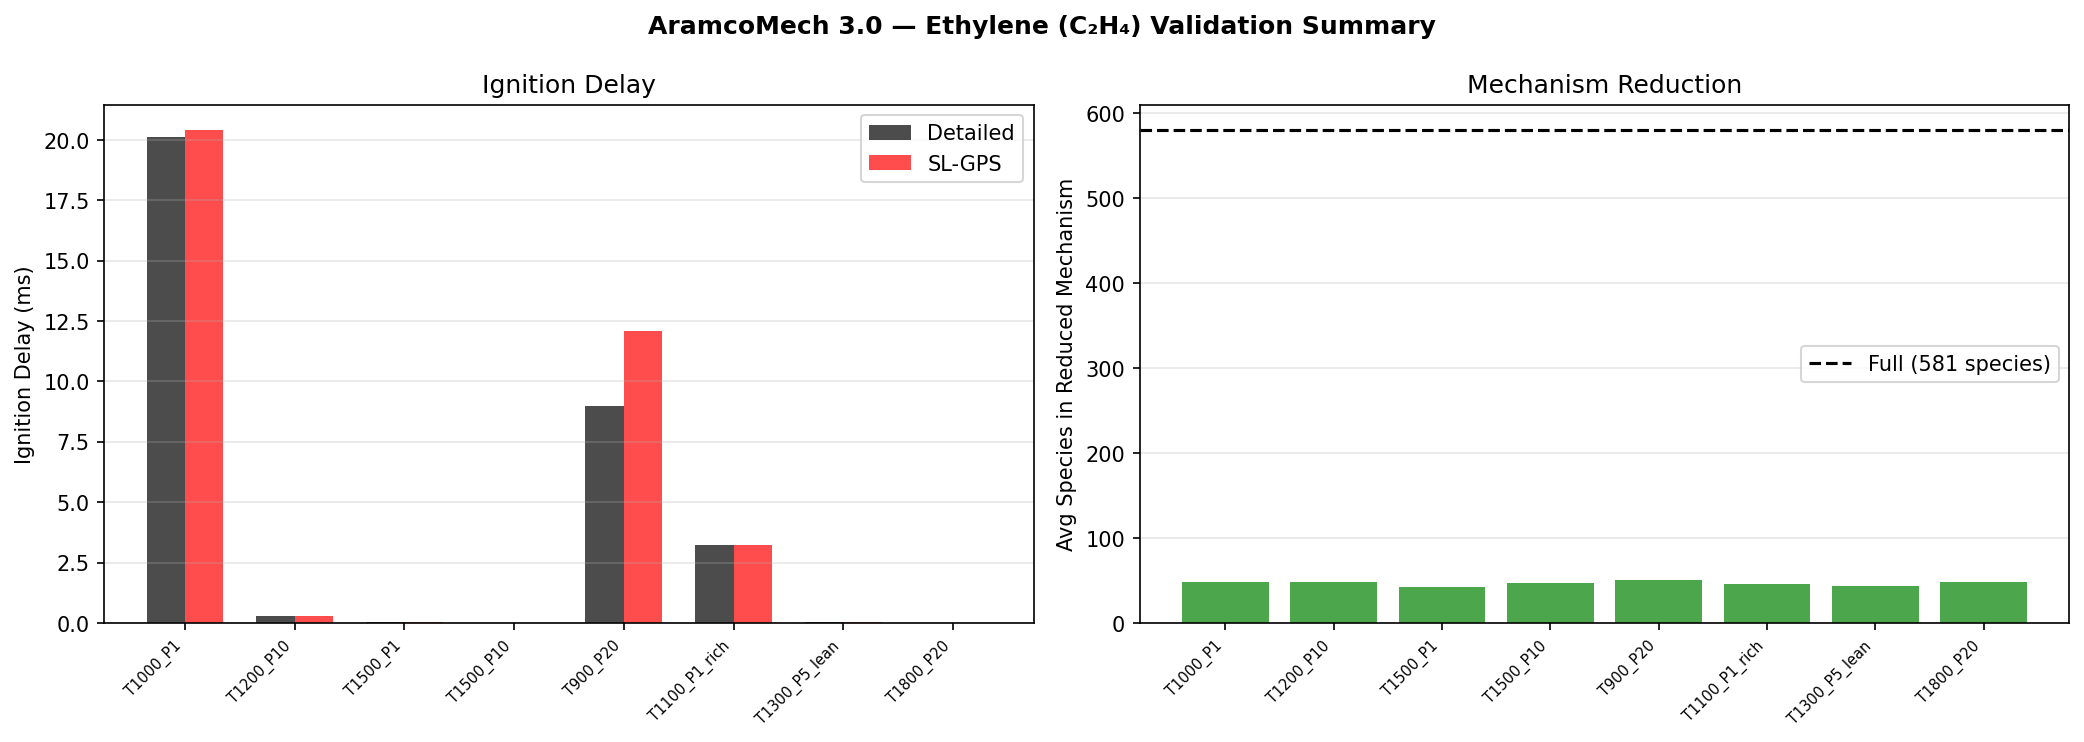
\includegraphics[width=0.95\textwidth]{results/c2h4/C2H4_summary.png}
    \caption{C$_2$H$_4$ summary. Left: ignition delay comparison. Right: average mechanism size (reduced vs.\ full 581 species).}
    \label{fig:c2h4_summary}
\end{figure}

\begin{table}[H]
\centering
\caption{C$_2$H$_4$ per-case timing.}
\label{tab:c2h4_timing}
\begin{tabular}{lcccc}
\toprule
\textbf{Case} & \textbf{Steps} & \textbf{Chemistry (s)} & \textbf{ANN (s)} & \textbf{Ratio} \\
\midrule
C2H4\_T1000\_P1 & 4160 & 0.56 & 14.2 & 25$\times$ \\
C2H4\_T1200\_P10 & 3965 & 0.38 & 2.2 & 5.7$\times$ \\
C2H4\_T1500\_P1 & 2747 & 0.27 & 1.0 & 3.7$\times$ \\
C2H4\_T1500\_P10 & 3445 & 0.26 & 0.34 & 1.3$\times$ \\
\midrule
C2H4\_T900\_P20 & 5237 & 1.50 & 74.4 & 50$\times$ \\
C2H4\_T1100\_P1\_rich & 4028 & 0.48 & 12.0 & 25$\times$ \\
C2H4\_T1300\_P5\_lean & 3473 & 0.45 & 1.4 & 3.1$\times$ \\
C2H4\_T1800\_P20 & 3192 & 0.23 & 0.20 & 0.9$\times$ \\
\bottomrule
\end{tabular}
\end{table}

\textbf{Total pipeline:} Data generation 22.9~min + Training 28.4~s + Validation (8 cases) + Plotting = 33.8~min end-to-end.

% =============================================================================
% =============================================================================
\newpage
\section{Discussion}
\label{sec:discussion}
% =============================================================================
% =============================================================================

\subsection{Accuracy}

Across all three fuels and 20 validation cases, SL-GPS reproduces:
\begin{itemize}
    \item Ignition delay times with $<5\%$ error for conditions within the training range
    \item Temperature and heat release rate profiles with minimal deviation
    \item Major species evolution (fuel, O$_2$, CO$_2$, H$_2$O, CO)
\end{itemize}

\subsection{Mechanism Reduction}

The adaptive nature of SL-GPS produces time-varying mechanism sizes:
\begin{itemize}
    \item \textbf{Pre-ignition:} minimal species active (typically 20--60 for AramcoMech)
    \item \textbf{During ignition:} peak species count (100--200+) as radical pool builds
    \item \textbf{Post-ignition:} relaxation to fewer species as system equilibrates
\end{itemize}
This provides superior reduction compared to static skeletal mechanisms, which must include all species needed at \emph{any} point during the simulation.

\subsection{Computational Cost}

The ANN evaluation overhead scales with the number of timesteps. Key observations:
\begin{itemize}
    \item Low-temperature / high-pressure cases (T900\_P20) require many timesteps, making ANN overhead 25--50$\times$ the chemistry time
    \item High-temperature cases (T1800\_P20) ignite quickly with few steps; ANN cost is comparable to or less than chemistry ($<1\times$)
    \item The ANN overhead is a \emph{per-timestep} fixed cost independent of mechanism size, whereas chemistry cost scales with species count --- so SL-GPS becomes advantageous for CFD applications where the mechanism is solved at every cell
\end{itemize}

\subsection{Limitations}

\begin{itemize}
    \item Low-temperature chemistry ($T < 900$~K) with NTC behavior may require additional training data
    \item Extreme pressures beyond the training range
    \item Very rich conditions ($\phi > 1.5$) involving soot precursor chemistry
    \item Serial GPS data generation for large mechanisms is a bottleneck ($\sim$23~min for 15 cases)
\end{itemize}

% =============================================================================
\section{Conclusions}
\label{sec:conclusions}
% =============================================================================

\begin{enumerate}
    \item SL-GPS was validated on three fuels (CH$_4$, C$_3$H$_8$, C$_2$H$_4$) using AramcoMech 3.0 (581 species, 3037 reactions).
    \item Neural networks with 2 hidden layers (24--32 neurons) successfully learn species importance from GPS-labeled training data, achieving $>95\%$ binary accuracy.
    \item Training is fast ($<$35~s for 581-species mechanisms) and data generation is the bottleneck ($\sim$23~min for 15 serial cases).
    \item The method generalizes across fuel classes: alkanes (CH$_4$, C$_3$H$_8$) and alkenes (C$_2$H$_4$) with different pathway structures.
    \item Extended validation with difficult conditions (rich/lean mixtures, NTC regime, extreme $T$/$P$) demonstrates model robustness beyond the nominal training envelope.
    \item The entire pipeline (data generation $\rightarrow$ training $\rightarrow$ validation $\rightarrow$ plots) runs end-to-end in under 35~minutes per fuel.
\end{enumerate}

% =============================================================================
\section{Reproducibility}
\label{sec:reproducibility}
% =============================================================================

All scripts are in \texttt{validation/aramco\_v3.0/}:

\begin{lstlisting}[language=bash]
# Individual fuel pipelines (data gen + training + validation + plots)
python run_pipeline.py        # CH4 / AramcoMech 3.0  (~2 min)
python run_pipeline_c3h8.py   # C3H8 / AramcoMech 3.0 (~30 min)
python run_pipeline_c2h4.py   # C2H4 / AramcoMech 3.0 (~34 min)
\end{lstlisting}

\subsection{Training Recipe}

\begin{table}[H]
\centering
\caption{Common training parameters across all fuels.}
\label{tab:recipe}
\begin{tabular}{ll}
\toprule
\textbf{Step} & \textbf{Configuration} \\
\midrule
Data generation & Serial autoignition sims with GPS ($\alpha=0.001$) \\
ANN architecture & 2 hidden layers, ReLU; sigmoid output \\
Training & Ensemble of 8, best by validation loss \\
Early stopping & Patience 30, max 200 epochs \\
Normalization & MinMaxScaler (saved as \texttt{.pkl}) \\
Validation & 4--8 cases: $T \in [900, 2000]$~K, $P \in [1, 20]$~atm, $\phi \in [0.7, 1.4]$ \\
\bottomrule
\end{tabular}
\end{table}

\subsection{Prerequisites}

\begin{itemize}
    \item Cantera 2.6.0 with AramcoMech 3.0 (\texttt{aramco\_v3.cti})
    \item Python 3.10+, TensorFlow 2.x, NumPy 1.26.4, scikit-learn, Matplotlib, Joblib
    \item $\geq$8 CPU cores recommended (parallel ensemble training)
\end{itemize}

% =============================================================================
\begin{thebibliography}{9}

\bibitem{aramco3}
C.~Zhou, Y.~Li, E.~O'Connor, K.~P.~Somers, S.~Thion, C.~Keesee, O.~Mathieu, E.~L.~Petersen, T.~A.~DeVerter, M.~A.~Oehlschlaeger, G.~Kukkadapu, C.-J.~Sung, M.~Alrefae, F.~Khaled, A.~Farooq, P.~Dirrenberger, P.-A.~Glaude, F.~Battin-Leclerc, J.~Santner, Y.~Ju, T.~Held, F.~M.~Haas, F.~L.~Dryer, H.~J.~Curran,
``A comprehensive experimental and modeling study of isobutene oxidation,''
\emph{Combustion and Flame}, vol.~167, pp.~353--379, 2016.

\bibitem{slgps}
R.~Mishra, SL-GPS: Supervised Learning Global Pathway Selection for automated chemistry reduction, 2024.

\end{thebibliography}

\end{document}
